\documentclass[conference]{IEEEtran}

\makeatletter
\def\endthebibliography{\def\@noitemerr{\@latex@warning{Empty `thebibliography' environment}}\endlist
}
\makeatother

\IEEEpeerreviewmaketitle

\usepackage{filecontents}
\usepackage[noadjust]{cite}
\usepackage{amsmath}
\usepackage{amssymb}
\usepackage{ebproof}
\usepackage{todonotes}
\usepackage{amsfonts}
\usepackage{algorithmic}
\usepackage{textcomp}
\usepackage{mathpartir}
\usepackage{color}
\usepackage{xcolor}
\DeclareMathAlphabet{\mathpzc}{OT1}{pzc}{m}{it}

\usepackage{subcaption} \usepackage{epsfig}
\usepackage{listings}
\usepackage[override]{cmtt}
\usepackage{graphicx}
\usepackage{balance}
\usepackage{xspace}
\usepackage{booktabs}
\usepackage{url}
\usepackage{xparse}
\usepackage{enumitem}
\usepackage{tikz}
\usetikzlibrary{chains,fit,shapes,positioning,calc,arrows.meta,shapes.arrows}

\usepackage[numbers]{natbib}
\bibliographystyle{plainnat}


\lstdefinestyle{customc}{
  belowcaptionskip=1\baselineskip,
  breaklines=true,
  numbers=left,
  xleftmargin=\parindent,
  language=C,
  columns=flexible,      
  showstringspaces=false,
  basicstyle=\small\sffamily,
  otherkeywords={uint},
  literate={{<-}{{$\leftarrow\,$}}2
            {->}{{$\rightarrow\,$}}2
            {<=}{{$\leq\,$}}2},
  numberstyle=\tiny\rmfamily,
  keywordstyle=\bfseries\color{green!40!black},
  commentstyle=\itshape\color{purple!40!black},
  identifierstyle=\color{blue!80!black},
}
\lstset{language=C,style=customc}

\newenvironment{DIFnomarkup}{}{}
\newcommand{\myparagraph}[1]{\textbf{#1}.\xspace}

\newcommand{\code}[1]{\lstinline|#1|}
%\newcommand{\ignore}[1]{{}}
\newcommand{\kwchecked}{\lstinline|\_Checked|}
\newcommand{\kwunchecked}{\lstinline|\_Unchecked|}
\newcommand{\kwdynamiccheck}{\lstinline|\_Dynamic\_check|}

\newcommand{\var}[1]{#1}
\newcommand{\Arrayptr}[1]{\lstinline|_Array_ptr<|{#1}\lstinline|>|}
\newcommand{\ArrayptrT}{\Arrayptr{$\tau$}}
\newcommand{\Ptr}[1]{\lstinline|_Ptr<|{#1}\lstinline|>|}
\newcommand{\PtrName}{\lstinline|_Ptr|}
\newcommand{\PtrT}{\Ptr{$\tau$}}
\newcommand{\Ntarrayptr}[1]{\lstinline|_Nt_array_ptr<|{#1}\lstinline|>|}
\newcommand{\NtarrayptrT}{\Ntarrayptr{$\tau$}}
\newcommand{\Checkedarr}[2]{{#1}~\lstinline|_Checked[|{#2}\lstinline|]|}
\newcommand{\CheckedarrT}[1]{\Checkedarr{$\tau$}{#1}}

\newif\ifsubmit\submitfalse

\ifsubmit
\newcommand{\mwh}[1]{}
\newcommand{\ashe}[1]{}
\newcommand{\dtarditi}[1]{}
\newcommand{\dvh}[1]{}
\newcommand{\leo}[1]{}
\newcommand{\liyi}[1]{}
\newcommand{\yiyun}[1]{}
\else
\newcommand{\mwh}[1]{\textcolor{red}{Mike: #1}}
\newcommand{\dtarditi}[1]{\textcolor{purple}{David: #1}}
\newcommand{\leo}[1]{\textcolor{green!80!blue}{Leo: #1}}
\newcommand{\liyi}[1]{\textbf{\textcolor{orange}{[ Liyi: #1 ]}}}
\newcommand{\yiyun}[1]{\textcolor{cyan}{Yiyun: #1}}
\newcommand{\dvh}[1]{\textcolor{magenta}{DVH: #1}}
\fi

\newcommand{\lang}{\textsc{CoreChkC}\xspace}
\newcommand{\elang}{\textsc{CoreC}\xspace}

\newtheorem{defi}{Definition}
\newtheorem{thm}{Theorem}
\newtheorem{prop}{Proposition}


\newcommand{\CoreChkC}{\textsc{CoreChkC}\xspace}
\newcommand{\checkedc}{\text{Checked C}\xspace}

 \newcommand{\rulelab}[1]{{\small \textsc{#1}}}
\newcommand{\steps}{\ensuremath{\longrightarrow}}
\newcommand{\tbool}{\texttt{bool}}
\newcommand{\tsizeof}{\texttt{sizeof}}
\newcommand{\vbool}{\texttt{Bool}}
\newcommand{\verror}{\texttt{Error}}
\newcommand{\vval}{\mathpzc{val}}
\newcommand{\tfixed}{\texttt{fixedp}}
\newcommand{\tnat}{\texttt{nat}}
\newcommand{\tarr}[2]{\texttt{array}~{#1}~{#2}}
\newcommand{\econst}[2]{({#1}){#2}}
\newcommand{\eindex}[2]{{#1}\texttt{[}{#2}\texttt{]}}
\newcommand{\sassign}[4]{{#1} \leftarrow {#3}~{#2}~{#4}}
\newcommand{\ssassign}[3]{{#1} \xleftarrow{#2} {#3}}
\newcommand{\sif}[3]{\texttt{if}~{#1}~{#2}~{#3}}
\newcommand{\sfor}[3]{\texttt{for}~{#1}~{#2}~{#3}}
\newcommand{\scall}[3]{{#1}\leftarrow {#2}~{#3}}
\newcommand{\sseq}[2]{{#1}\,\texttt{;}\,{#2}}
\newcommand{\sinv}[1]{\texttt{inv}~{#1}}
\newcommand{\inst}[3][ ]{\texttt{#2}^{#1}~{#3}}
\newcommand{\insttwo}[4][ ]{\texttt{#2}^{#1}~{#3}~{#4}}
\newcommand{\instthree}[5][ ]{\texttt{#2}^{#1}~{#3}~{#4}~{#5}}
\newcommand{\iskip}[1]{\inst{ID}{#1}}
\newcommand{\inot}[1]{\inst{X}{#1}}
\newcommand{\ictrl}[2]{\insttwo{CU}{#1}{#2}}
\newcommand{\irz}[3][ ]{\insttwo[#1]{RZ}{#2}{#3}}
\newcommand{\isr}[3][ ]{\insttwo[#1]{SR}{#2}{#3}}
\newcommand{\icnot}[2]{\insttwo{CNOT}{#1}{#2}}
\newcommand{\ilshift}[1]{\inst{Lshift}{#1}}
\newcommand{\irshift}[1]{\inst{Rshift}{#1}}
\newcommand{\irev}[1]{\inst{Rev}{#1}}
\newcommand{\iqft}[2][ ]{\inst[#1]{QFT}{#2}}
\newcommand{\ihad}[1]{\inst{H}{#1}}

\newcommand{\iseq}[2]{{#1}\,\texttt{;}\,{#2}}
\newcommand{\inval}[2]{\insttwo{Nval}{#1}{#2}}
\newcommand{\ihval}[3]{\instthree{Hval}{#1}{#2}{#3}}
\newcommand{\iqval}[2]{\insttwo{Qval}{#1}{#2}}

\newcommand{\instr}{\iota}

\newcommand{\kw}[1]{\ensuremath{\mathtt{#1}}}
\newcommand{\subtype}[2]{\ensuremath{\vdash{#1}\prec{#2}}}
\newcommand{\estrlen}[1]{\ensuremath{\kw{strlen}({#1})}}
\newcommand{\estrlentext}{\ensuremath{\kw{strlen}}}

\newcommand{\tarray}[3]{\tarrayb{({#1},{#2})}{#3}}
\newcommand{\tarrayb}[2]{\ensuremath{[{#1}~{#2}]}}
\newcommand{\tntarray}[3]{\tntarrayb{({#1},{#2})}{#3}}
\newcommand{\tntarrayb}[2]{\tarrayb{#1}{#2}_{nt}}
\newcommand{\tallarrayb}[2]{\ensuremath{[{#1}~{#2}]_{\kappa}}}
\newcommand{\tallarraybc}[2]{\ensuremath{[{#1}~{#2}]_{\textcolor{cyan}{\kappa}}}}

\newcommand{\tallarray}[3]{\tallarrayb{({#1},{#2})}{#3}}

\newcommand{\tptr}[2]{\ensuremath{\mathtt{ptr}^{#2}~{#1}}}
\newcommand{\tntptr}[4]{\ensuremath{[({#1},{#2})~{#3}]^{#4}_{nt}*}}


\newcommand{\tarrayptr}[4]{{\tptr{\tarray{#1}{#2}{#3}}{#4}}}
\newcommand{\tntarrayptr}[4]{{\tptr{\tntarray{#1}{#2}{#3}}{#4}}}
\newcommand{\tallarrayptr}[4]{{\tptr{\tallarray{#1}{#2}{#3}}{#4}}}


\newcommand{\tgarray}[4]{\ensuremath{\mathtt{#1}~{#2}~{#3}~{#4}}}
\newcommand{\tstruct}[1]{\ensuremath{\kw{struct}~{#1}}}

\newcommand{\evalue}[2]{\ensuremath{{#1}\!:\!{#2}}}

\newcommand{\emalloc}[1]{\ensuremath{\kw{malloc}({#1})}}
\newcommand{\emalloctext}{\ensuremath{\kw{malloc}}}
\newcommand{\ecall}[2]{\ensuremath{{#1}({#2})}}
\newcommand{\ret}[3]{\ensuremath{\kw{ret}({#1},{#2},{#3})}}
\newcommand{\rettext}{\ensuremath{\kw{ret}}}
\newcommand{\ecast}[2]{\ensuremath{\kw{(}{#1}\kw{)}{#2}}}
\newcommand{\edyncast}[2]{\ensuremath{\langle{#1}\rangle{#2}}}
\newcommand{\edcast}[2]{\ensuremath{\kw{(D},{#1}\kw{)}{#2}}}
\newcommand{\elet}[3]{\ensuremath{\kw{let}~#1\, \texttt{=}\, #2~\kw{in}\;{#3}}}
\newcommand{\elettext}{\ensuremath{\kw{let}}}
\newcommand{\ebinop}[2]{\ensuremath{#1 \plus #2}}
\newcommand{\eassign}[2]{\ensuremath{\texttt{*}{#1}\,\texttt{=}\, {#2}}}
\newcommand{\eassignstack}[2]{\ensuremath{{#1}\,\texttt{=}\, {#2}}}
\newcommand{\efield}[2]{\ensuremath{{#1}\kw{\rightarrow}{#2}}}
\newcommand{\estar}[1]{\ensuremath{\texttt{*}{#1}}}
\newcommand{\eamper}[2]{\ensuremath{\kw{\&}{#1}\kw{\rightarrow}{#2}}}
\newcommand{\eunchecked}[1]{\ensuremath{\kw{unchecked}\;{#1}}}
\newcommand{\euncheckedtext}{\ensuremath{\kw{unchecked}}}
\newcommand{\eif}[3]{\ensuremath{\kw{if\;}(#1)\;{#2}\;\kw{else}\;{#3}}}
\newcommand{\eifa}[3]{\ensuremath{\kw{IF\;}(#1)\;{#2}\;\kw{ELSE}\;{#3}}}
\newcommand{\eifatext}{\ensuremath{\kw{IF}}}

\newcommand{\eiftext}{\ensuremath{\kw{if}}}
\newcommand{\ethentext}{\ensuremath{\kw{then}}}
\newcommand{\eelse}{\ensuremath{\kw{else}}}
\newcommand{\ebreak}{\ensuremath{\kw{break}}}
\newcommand{\ebounds}{\ensuremath{\kw{bounds}}}
\newcommand{\enull}{\ensuremath{\kw{null}}}
\newcommand{\hole}{\ensuremath{\Box}}
\newcommand{\defscope}{\sigma}
\newcommand{\wf}[1]{wf \, #1}
\newcommand{\tint}{\ensuremath{\mathtt{int}}}
\newcommand{\efor}{\ensuremath{\mathtt{for}}}
\newcommand{\ewhile}{\ensuremath{\mathtt{while}}}
\newcommand{\etrue}{\ensuremath{\mathtt{true}}}
\newcommand{\efalse}{\ensuremath{\mathtt{false}}}
\newcommand{\edplus}{\ensuremath{\texttt{++}}}
\newcommand{\edminus}{\ensuremath{\texttt{--}}}

\newcommand{\ememcpy}{\ensuremath{\mathtt{memcpy}}}
\newcommand{\ereturn}{\ensuremath{\mathtt{return}}}
\newcommand{\emain}{\ensuremath{\mathtt{main}}}
\newcommand{\estrcat}{\ensuremath{\mathtt{strcat}}}
\newcommand{\estrcatbad}{\ensuremath{\mathtt{strcat\_b}}}
\newcommand{\heap}{\ensuremath{\mathpzc{H}}}
\newcommand{\eret}[3]{\ensuremath{\kw{ret}({#1},{#2},{#3})}}
\newcommand{\erettext}{\ensuremath{\kw{ret}}}

\newcommand{\plus}{\mathbin{\texttt{+}}}

\newcommand{\fv}{\mathit{FV}}
\newcommand{\dom}{\mathit{dom}}

\newcommand{\fm}{\mathit{FM}}
\newcommand{\size}{\mathit{size}}

\newcommand{\cmode}{\texttt{c}}
\newcommand{\umode}{\texttt{u}}
\newcommand{\bvar}{\ensuremath{\beta}}
\newcommand{\mode}{\textit{mode}}

\newcommand{\cextend}[4]{\ensuremath{#4 = ~ \vdash_{extend} #1, #2, #3}}
\newcommand{\fresh}{\ensuremath{\kw{fresh}}}
\newcommand{\echecknull}[3]{\ensuremath{#3 = ~\vdash_{null}#1, #2}}
\newcommand{\echeckboundsdyn}[5]{\ensuremath{#5 = ~ \vdash_{boundsD}#1, #2, #3, #4}}
\newcommand{\echeckbounds}[5]{\ensuremath{#5 = ~ \vdash_{boundsR}#1, #2, #3, #4}}
\newcommand{\echeckboundsw}[5]{\ensuremath{#5 = ~ \vdash_{boundsW}#1, #2, #3, #4}}
\newcommand{\esizeof}[1]{\ensuremath{\kw{sizeof}(#1)}}
\newcommand{\ewidenstrlen}[5]{\ensuremath{#5 = ~ \vdash_{widenstr}#1, #2, #3, #4}}
\newcommand{\ewidenderef}[4]{\ensuremath{#4 = ~ \vdash_{widenderef}#1, #2, #3}}
\newcommand{\eleq}[2]{\ensuremath{#1 \leq #2}}




\newcommand{\rboundle}[2]{\ensuremath{\vdash_{bounds}#1 \leq #2}}








\def\codesize{\normalsize}
\definecolor{programs}{gray}{0.1}

\lstset{
  basicstyle=\ttfamily,  
}

\makeatletter
\lst@CCPutMacro
    \lst@ProcessOther {"22}{\lst@ifupquote \textquotedbl
                                     \else \char34\relax \fi}
    \@empty\z@\@empty
\makeatother

\lstloadlanguages{C}

\def\BibTeX{{\rm B\kern-.05em{\sc i\kern-.025em b}\kern-.08em
    T\kern-.1667em\lower.7ex\hbox{E}\kern-.125emX}}
\begin{document}

\title{A Formal Model of Checked C}         




% \ignore{
% \author{\IEEEauthorblockN{1\textsuperscript{st} Leonidas Lampropoulos}
% \IEEEauthorblockA{\textit{Department of Computer Science} \\
% \textit{University of Maryland}\\
% llampro@cs.umd.edu}
% \and
% \IEEEauthorblockN{1\textsuperscript{st} Michael Hicks}
% \IEEEauthorblockA{\textit{Department of Computer Science} \\
% \textit{University of Maryland}\\
% llampro@cs.umd.edu}
% }
% \author{Leonidas Lampropoulos \and
% Michael Hicks}
% }
\maketitle

\begin{abstract}


  We present a formal model of Checked C, a dialect of C
  that aims to enforce spatial memory safety. Our model pays particular
  attention to the semantics of dynamically sized, potentially null-terminated
  arrays.
We formalize this model in Coq, and prove that any spatial memory
  safety errors can be \emph{blamed} on portions of the program
  labeled \emph{unchecked}; this is a Checked C feature that supports
  incremental porting and backward compatibility.
Our model develops an operational semantics that uses fat pointers to
  guarantee spatial safety. However, we formalize a compilation scheme
  that can yield thin pointers, with bounds information managed using
  inserted code. We show that the generated code faithfully simulates
  the original.
Finally, we build an executable version of our model in PLT Redex, 
  and use a custom random generator
  for well-typed and almost-well-typed terms to find
  inconsistencies between our model and the Clang Checked C
  implementation. We find these steps to be a useful way to co-develop a language
  (Checked C is still in development) and a core model of it.
\end{abstract}



\section{Introduction}\label{sec:intros}

The C programming language remains extremely popular despite the
emergence of new, modern languages. Unfortunately, C programs lack
spatial memory safety, which makes them susceptible to a host
of devastating vulnerabilities, including buffer overflows and
out-of-bounds reads/writes. Despite their long history, buffer
overflows and other spatial safety violations are among the most
prevalent and dangerous vulnerabilities on the Internet today \cite{Zeng:2013:SRF:2534766.2534798}.



Several industrial and research efforts---including CCured~\cite{Necula2005},
Softbound~\cite{softbound}, and ASAN~\cite{Serebryany2012}---have
explored means to compile C programs 
to automatically enforce spatial safety. These
approaches all impose performance overheads that are deemed too high for
use in deployment. Recently, Microsoft introduced \checkedc, an
open-source extension to C with new types and
annotations whose use can ensure a program’s spatial
safety~\cite{Elliott2018}. Importantly, \checkedc supports development that is
incremental and compositional. Code regions (e.g.,
functions or whole files) designated as \emph{checked} are sure to enforce
spatial safety, a property which is preserved via composition with
other checked regions. But not all regions must be checked: Checked
C's annotated \emph{checked pointers} are binary-compatible with legacy pointers, and
may coexist in the same code, which permits a deliberate (and
semi-automated) refactoring process. Parts of the FreeBSD kernel have
been successfully ported to \checkedc~\cite{duanrefactoring}, and overall, performance
overhead seems low enough for practical deployment.

While \checkedc promises to enforce spatial safety, we might wonder
whether its design and implementation deliver on this promise, or even
what ``spatial safety'' means when a program contains both checked and
unchecked code. In prior work, \citet{ruef18checkedc-incr} developed a core
formalization of \checkedc and with it proved that \emph{checked code cannot 
  be blamed}: any spatial safety violation can only be attributed to
code that is not in a checked region. While their work is a good start,
it fails to model important aspects of \checkedc's functionality,
particularly those involving pointers to arrays. In this paper, we
cover this gap, making three main contributions.

\myparagraph{Dynamically bounded and null-terminated arrays}
Our first contribution is a core formalism called \lang, which extends
\citet{ruef18checkedc-incr} with several new features, most notably 
\emph{dynamically bounded arrays} (Section~\ref{sec:formal}). 
Dynamically bounded arrays are those whose size is
known only at run time, as designated by in-scope variables using
dependent types. A pointer's accessible memory is bounded both above
and below, to admit arbitrary pointer arithmetic.

\lang also models
\emph{null-terminated} arrays, a kind of dynamically bounded array whose upper bound 
defines the array's \emph{minimum} length---additional space is available 
up to a null terminator. For example, the \checkedc type
\lstinline{nt_array_ptr<char> p:count(n)} says that
\lstinline{p} has length \emph{at least} \lstinline{n} (excluding the
null terminator), but further capacity is present if \lstinline|p[n]| is not null. \checkedc (and \lang) supports flow-sensitive
\emph{bounds widening}: statements of the form \lstinline|if (*p) | $s$,
where \lstinline{p}'s type is \lstinline{nt_array_ptr<T> count(0)},
typecheck statement $s$ under the assumption that \lstinline{p} has
type \lstinline{nt_array_ptr<T> count(1)}, 
 i.e., one more than it was,
since the character at the current-known length is
non-null. Similarly, the call \lstinline|n = strlen(p)| will widen
\lstinline|p|'s bounds to \lstinline|n|. Subtyping permits treating
null-terminated arrays as normal arrays of the same size (which
does not include, and thereby protects, the null terminator).

We prove, in Coq, a blame theorem for \lang.  As far as we are aware,
ours is the first formalized type system and proof of soundness for
pointers to null-terminated arrays with expandable bounds.



\myparagraph{Sound compilation of checked pointers} Our second
contribution is a formalization of bounds-check insertion for array
accesses (Section~\ref{sec:compilation}). Our operational semantics
annotates each pointer with metadata that describes its bounds, and
the assignment and dereference rules have premises to confirm the
access is in bounds. An obvious compilation scheme (taken by
Cyclone~\cite{Jim2002,GrossmanMJHWC02}, CCured~\cite{Necula2005}, and
earlier works) would be to translate annotated pointers to multi-word
objects: one word for the pointer, and 1-2 words to describe its lower
and upper bounds. Inserted checks reference these bounds. While
convenient, such ``fat'' pointers are expensive, and break backward
binary compatibility with legacy pointers. We formalize \checkedc's
compilation approach, which uses a single machine word for the
pointer, and adds checks involving the declared bounds (e.g., in a
dependent type) or additional stack-allocated \emph{ghost variables}
to accommodate bounds widening. We show that the compiled program
\emph{simulates} the original by mechanizing \lang and the compilation
judgment in PLT Redex~\cite{pltredex}, and use its random testing
feature to give confidence that simulation holds.


As far as we are aware, \lang is the first formalism to cleanly
separate bounds-checking compilation from the core semantics; prior
work merged the two, conflating \emph{meaning} with
\emph{mechanism}~\cite{Feng2006,Condit2007}. In carrying out the 
formalization, we discovered that our compilation approach is 
more expressive than that proposed in the Checked C
specification~\cite{checkedc} (Section~\ref{sec:disc}); we 
would not have discovered this improvement had we not separated checks from 
semantics. 





\myparagraph{Model-based randomized testing} Our third
and final contribution is a strategy and implementation of model-based
randomized testing (Section~\ref{sec:evaluation}).  To check the
correctness of our formal model, we compare the behavior between the
existing Clang \checkedc implementation and our own model. This is
done by a conversion tool that converts expressions from \lang into
actual \checkedc code that can be compiled by the Clang \checkedc
compiler. We build a random generator of programs largely based on the
typing rules of \lang and make sure that, both statically and
dynamically, \lang and Clang Checked C are consistent after
conversion.  This helped rapidly prototype the model and uncovered
several issues in the Checked C compiler.

We begin with a review of \checkedc (Section~\ref{sec:overview}),
present our main contributions (Sections~\ref{sec:formal}--\ref{sec:evaluation}),
and conclude with a discussion of
related and future work (Sections~\ref{sec:related}, \ref{sec:conclude}).








\section{\checkedc Overview}\label{sec:overview}

This section describes Checked C, which extends C with new pointer
types and annotations that ensure spatial safety. More
details can be found in a prior overview~\cite{Elliott2018} or the
full specification~\cite{checkedc}.
Checked C is implemented as a fork of Clang/LLVM and is freely
available.\footnote{\url{https://github.com/Microsoft/checkedc-clang}}

\begin{figure}[t]
{\small
  \begin{lstlisting}[xleftmargin=4 mm]
nt_array_ptr<const char>
parse_utf16_hex(nt_array_ptr<const char> s,
                  ptr<uint> result) {
 int x1, x2, x3, x4;
 if (s[0] != 0) { x1 = hex_char_to_int(s[0]);
 if (s[1] != 0) { x2 = hex_char_to_int(s[1]);
 if (s[2] != 0) { x3 = hex_char_to_int(s[2]);
 if (s[3] != 0) { x4 = hex_char_to_int(s[3]);
 if (x1 != -1 && x2 != -1 && x3 != -1 && x4 != -1){
   *result = (uint)((x1<<12)|(x2<<8)|(x3<<4)|x4);
   return s+4;
  ...// several } braces
 } 
 return 0;
}
void parse(nt_array_ptr<const char> s,
            array_ptr<uint> p : count(n), 
            int n) {
 array_ptr<uint> q : bounds(p,p+n) = p;
 while (s && q < p+n) {
   array_ptr<uint> r : count(1) =
     dyn_bounds_cast<array_ptr<uint>>(q,count(1));
   s = parse_utf16_hex(s,r);
   q++;
 }
}
  \end{lstlisting}

}

\caption{Parsing a string of UTF16 hex characters in \checkedc}
\label{fig:checkedc-example}
\end{figure}





\subsection{Checked Pointer Types}
\checkedc introduces three varieties of \emph{checked pointer}:
\begin{itemize}
\item \code{ptr<}$T$\code{>} types a pointer that is either null or
  points to a single object of type $T$.
\item \code{array_ptr<}$T$\code{>} types a pointer that is either null
  or points to an array of $T$ objects. The array width is defined
  by a \emph{bounds} expression, discussed below.
\item \code{nt_array_ptr<}$T$\code{>} is like
  \code{array_ptr<}$T$\code{>} except that the bounds expression
  defines the \emph{minimum} array width---additional objects may
  be available past the upper bound, up to a null terminator.
\end{itemize}
A bounds expression used with the latter two pointer types has three
forms:
\begin{itemize}
\item \code{count(}$e$\code{)} where $e$ defines the array's
  length. Thus, if pointer $p$ has bounds \code{count(n)} then the
  accessible memory is in the range $[p,p+$\code{n}$]$. Bounds
  expression $e$ must be side-effect free and may only refer to
  variables whose addresses are not taken, or adjacent \code{struct}
  fields.
\item \code{byte_count(}$e$\code{)} is like \code{count}, but
  expresses arithmetic using bytes, no objects; i.e.,
  \code{count(}$e$\code{)} used for \code{array_ptr<}$T$\code{>} is
  equivalent to \code{byte_count(}$e\times\texttt{sizeof}(T)$\code{)}
\item \code{bounds(}$e_l$,$e_h$\code{)} where $e_l$ and $e_h$ are
  pointers that bound the accessible region $[e_l,e_h)$ (the
  expressions are similarly restricted). Bounds
  \code{count(}$e$\code{)} is shorthand for
  \code{bounds(}$p, p + e$\code{)}. This most general form of bounds
  expression is useful for supporting pointer arithmetic.
\end{itemize}
The \checkedc compiler will instrument loads and stores of checked
pointers to confirm the pointer is non-null, and the access is within
the specified bounds. For pointers $p$ of type
\code{nt_array_ptr<}$T$\code{>}, such a check could spuriously fail if
the index is past $p$'s specified upper bound, but before the null
terminator. To address this problem, Checked C supports \emph{bounds
  widening}. If $p$ has bounds expression
\code{bounds(}$e_l$,$e_h$\code{)} a program may read from (but not
write to) $e_h$; when the compiler notices that a non-null character
is read at the upper bound, it will extend that bound to $e_h+1$.

\subsection{Example}

Fig.~\ref{fig:checkedc-example} gives an example \checkedc
program.\footnote{Ported from the Parson JSON
parser, \url{https://github.com/kgabis/parson}} 
The function \code{parse_utf16_hex} on lines 1-17 takes as its argument
null-terminated pointer \code{s} from which it attempts to read four
characters. These are interpreted as hex digits and converted to an
\code{uint} returned via parameter \code{result}. At first,
\code{s} has no specific bounds annotation, which we can interpret as
\code{count(0)}; this means that \code{s[0]} may be read on line
5. The true branch of the conditional (which extends all the way to
the brace on line 15) is thus typechecked with \code{s} given a
\emph{widened} bound of \code{count(1)}. Likewise, the conditionals on
lines 6-8 each widen it one further; the widened pointer
(\code{s+4}) is returned on success.

The \code{parse} function on lines 18-26 repeatedly invokes
\code{parse_utf16_hex} with its parameter \code{s}, and fills out
array \code{p} whose declared length is the parameter \code{n}. Writes
happen via pointer \code{q}, which is updated using pointer
arithmetic. We specify its bounds as
\code{bounds(p,p+n)} to support this: even as \code{q} changes, 
variables \code{p} and \code{n} do not. Converting from an
\code{array_ptr<uint>} to a \code{ptr<uint>}, done for the call on
line 25, requires proving the array has size at least 1. While this is true
because of the loop condition \code{q < p+n}, which is \code{q}'s
upper bound, the compiler is not smart enough to figure this
out. To convince it, we manually insert a bounds check using
\code{dyn_bounds_cast}.

While bounds checks are \emph{conceptually} inserted on every array
load and store, many of these are eliminated by LLVM\@. For example,
all of the pointer accesses to \code{s} on lines 5-8 are proved safe
at compile-time, so no bounds checks are inserted for
them. \citet{Elliott2018}
reported average run-time overheads of 8.6\% on a pointer-intensive
benchmark suite (49.3\% in one case); \citet{duanrefactoring} measured
no overhead at all on a port of FreeBSD's UDP and IP stacks to \checkedc.



\subsection{Other features}

\checkedc has other features not modeled in this paper. Two in regular
use are \emph{interop types}, which ascribe checked pointer types to
unported legacy code, notably in libraries; and \emph{generic types}
on both functions and \code{struct}s, for type-safe polymorphism. More
details about these can be found in the language specification.

\subsection{Spatial Safety and Backward Compatibility}
\checkedc is backward compatible with legacy C in the sense that all
legacy code will typecheck and compile. However, only code that
appears in \emph{checked regions}, which we call \emph{checked code},
is spatially safe. Checked regions can be designated at the level of
files, functions, or individual code blocks, the first with a
\code{#pragma} and the latter two using the \code{checked}
keyword.\footnote{You can also designate \emph{unchecked} regions
  within checked ones.}  Within checked regions, both
legacy pointers and certain unsafe idioms (e.g., variadic function
calls) are disallowed. The code in Fig.~\ref{fig:checkedc-example}
satisfies these conditions, and will typecheck in a checked region.

How should we think about code that contains both checked and legacy
components? \citet{ruef18checkedc-incr} proved, for a simple
formalization of \checkedc, that \emph{checked code cannot be blamed}:
Any spatial safety violation owes to the execution of unchecked
code. In this paper we extend that result to a richer formalization of
\checkedc. 





% \ignore{
% \liyi{Good information about pointer types here:
% https://github.com/microsoft/checkedc/wiki/New-pointer-and-array-types}




% This code creates an array pointer of length $10$, and reads the pointer $(x+y)$. 
% If the integer value $y$ is greater than $10$, executing the program in C results in undefined behavior. 
% In \checkedc, however, we links every pointer in a program with their bound information statically, and inserts checks to dynamically verify if the usage of the pointer violates the spatial safety. For example, In compiling the above fragment, we inserts the bound's check for $x$ in the read operation $(x+y)$, and if $y$ results in a value $11$, the execution of the read operation $(x+y)$ results in an dynamic error. 

% There are many existing language development trying to guarantee the C spatial safety property through different approaches. For example, Cyclone \cite{Jim2002} and Cerberus \cite{cerberus} are the fat pointer approaches for guaranteeing the spatial safety and eliminating undefined behaviors in C. Rust \cite{Rust2016}, on the other hand, tries to restrict the possible way of writing programs to guarantee such property statically.
% The problem of these two approaches are effectiveness of executing programs and user practicality of writing programs. The fat-pointer approach completely relies on dynamic checks to guarantee the safety properties but it might pay a huge price on execution efficiency. In our experiment (Sec.\ref{sec:evaluation}), we found that the execution of fat pointer approaches cost the speed a 50\% overhead. 
% On the other hand, Rust uses a static approach by restricting the usage of pointers to guarantee the properties, which results in a user UN-friendly system.  
% The development of \checkedc is an investigation on keeping the balance between execution efficiency and user-friendly systems. We develop a system to utilize static type systems to allow the \checkedc compiler to insert dynamic checks to guarantee the safety property. The efficiency of \checkedc is in the same level of Rust while we maintain a user-friendly system and inherited most of the operation features from C.

% Another feature of \checkedc is the division of the checked and unchecked blocks. When users try to rewrite their C programs into \checkedc programs, they can develop the code incrementally by rewriting sub-parts of their programs to \checkedc code fragments and placing them as the checked blocks, while keeping the rest C programs as unchecked C programs. \checkedc guarantees that if there is any safety violation, this comes from the unchecked blocks (the blame theory). 

% Here is the contributions of the paper. First, we develop the code formalization of \checkedc and show that the type system in \checkedc is type-sound and satisfies the blame theory with respect to the \checkedc semantics. Specifically, we formalize null-terminated array pointers. To our best knowledge, this is the first work defining such feature in C-related languages. 
% Second, in formalizing the \checkedc language, we investigate the balance between program execution efficiency and user practicality. We re-investigate the \checkedc type system with subtyping relations to make it more efficient and user-friendly.
% Second, we also develop random testing tools in Redex \cite{pltredex} to test the \checkedc compiler and make sure it is properly developed. We are able to find and reproduce many bugs/faults in the \checkedc compiler \liyi{numbers?}. The random testing tool is able to generate tens of thousands of programs to properly validate the \checkedc compiler. Third, we also spent a great amount of work in developing experiments to compare \checkedc and other existing C-like languages that guarantee the spatial safety and eliminating undefined behaviors. We found that \checkedc keeps the best balance between execution efficiency and user practicality.
% }



 
% \ignore{
% \section{Null-Terminated Array Pointers}

% Key ideas, formalized:
% \begin{itemize}
% \item Can read one past the end: x[N] can be read, but only written if
%   the value being written is 0.
% \item NT arrays are a refinement of normal arrays: Can convert
%   x:(ntarray N t) to (array N t).
% \item NT arrays can expand their length flow sensitively: Can convert
%   x:(ntarray N t) to (ntarray N+1 t) assuming x[N] != 0.
% \item In general unsafe to convert x:(array N t) to (ntarray N-1 t)
%   even if x[N-1] == 0 because aliases of x could eliminate the NULL
%   terminator. Would need some sort of linearity/alias tracking to
%   support this idea.
% \item Question? What is the syntax of doing a malloc on a NT-array?
%   Should we just do malloc(NT-array l h type) as the malloc of a
%   normal array or should we also include something like int [] nt =
%   “abcd”, where the bound size is not specified?
% \end{itemize}

% See also the Checked C specification
% \ignore{
% https://github.com/microsoft/checkedc/tree/master/spec/bounds\_safety}
% }

\section{Formalization}\label{sec:formal}

















% \ignore{
% \begin{figure}
%   \begin{center}
%     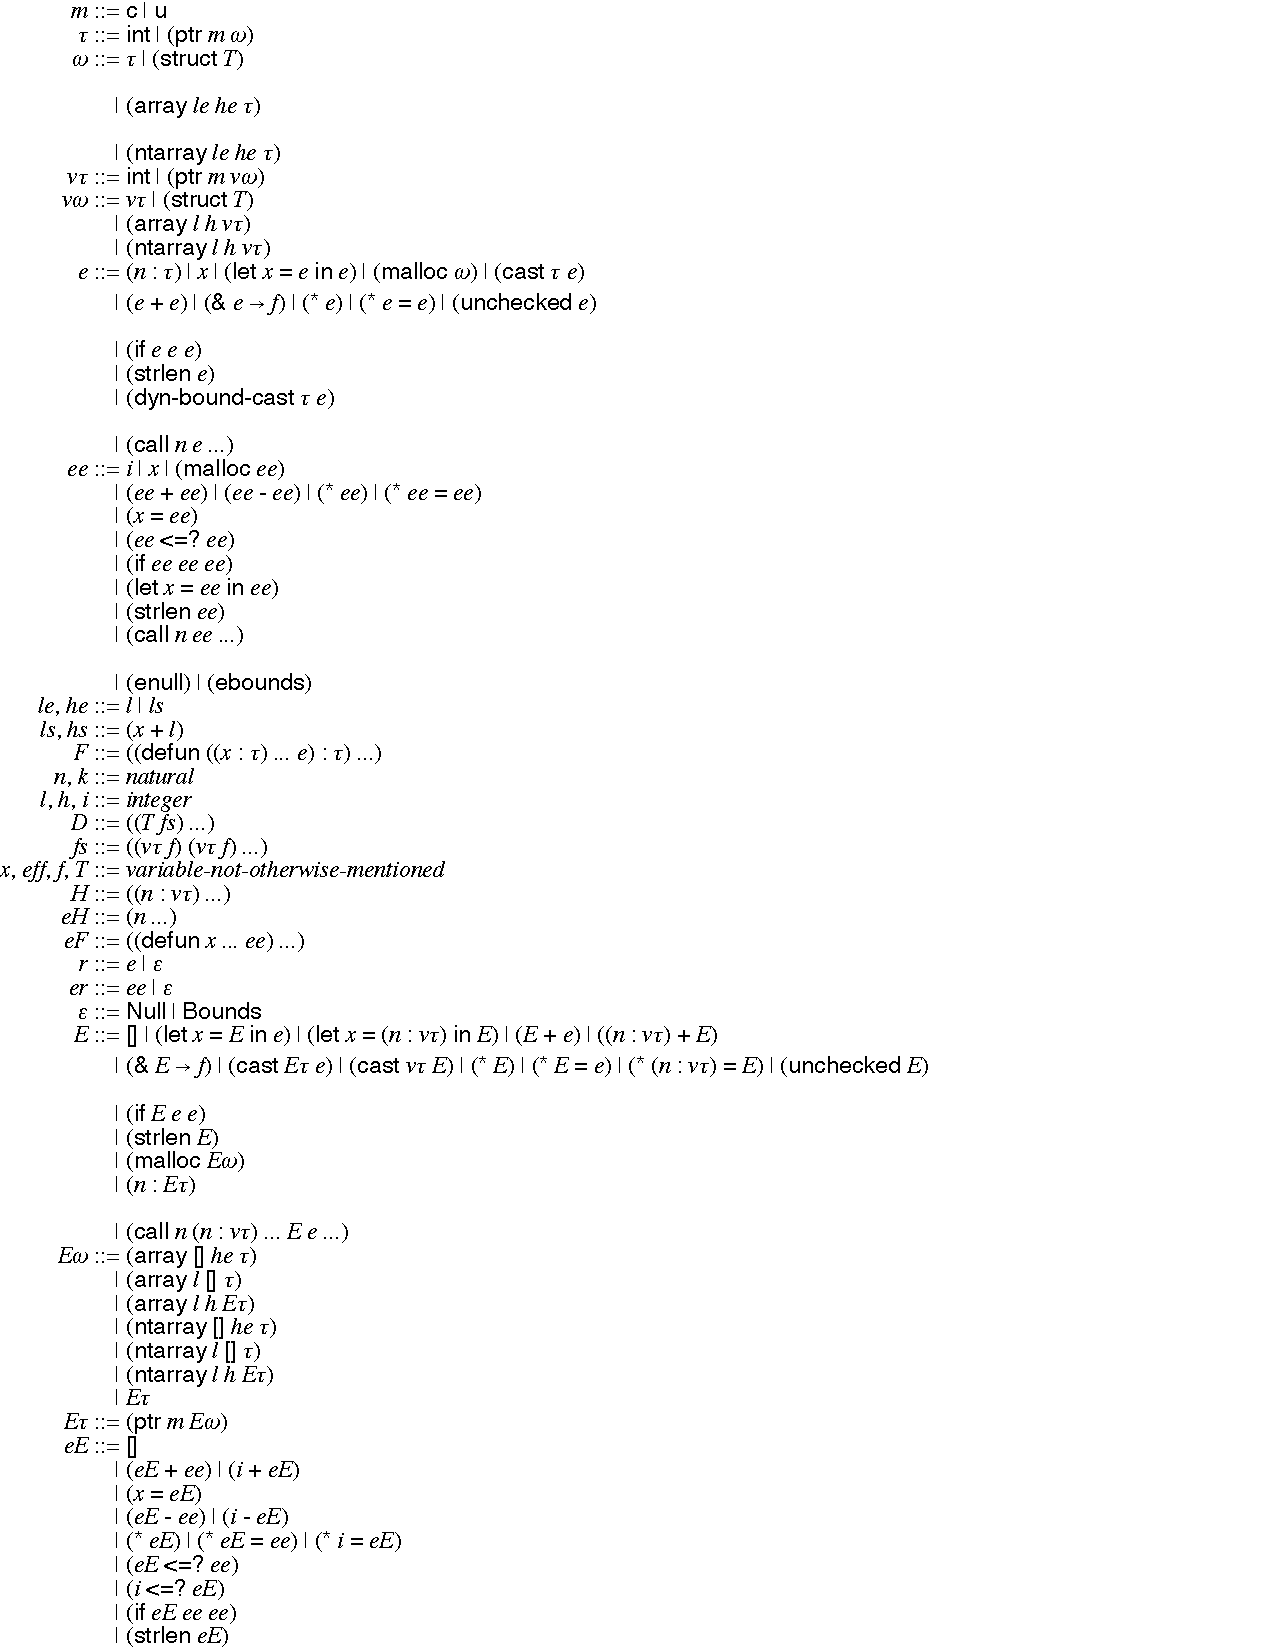
\includegraphics[height=6in]{syntax.pdf}
%   \end{center}
%   \caption{\lang: Syntax}
% \end{figure}

% \begin{figure}
%   \begin{center}
%     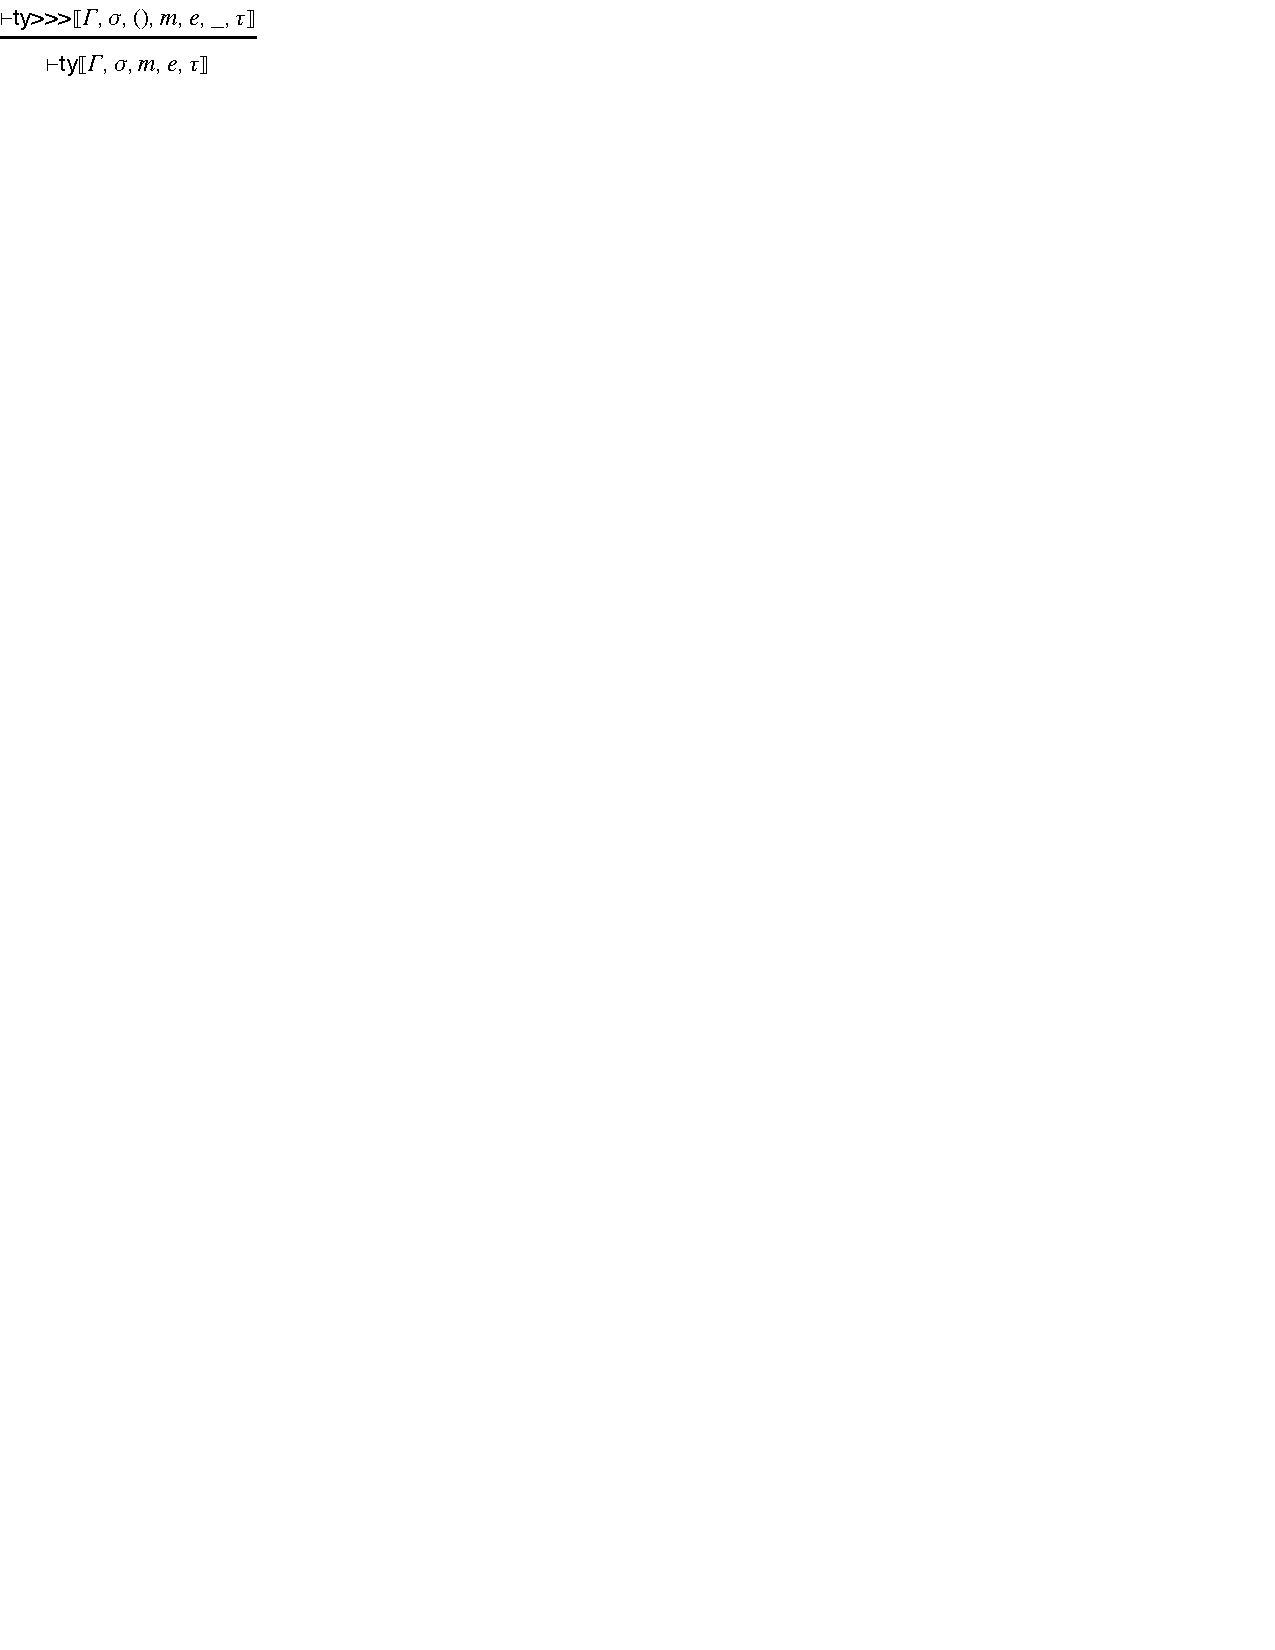
\includegraphics[height=6in]{types.pdf}
%   \end{center}
%   \caption{\lang: Typing}
% \end{figure}
% }





\begin{figure}
  \small \centering
  $\begin{array}{l}
\begin{array}{lll}
\text{Function names:}~f&
       \text{Variables:}~ x
& \text{Integers:}~n::=\mathbb{Z} 
\end{array}
\\[0.5em]

\begin{array}{llcllcl}

\text{Mode:} & m & ::= & \cmode \mid \umode \\[0.5em]

\text{Bound:} & b & ::= & n \mid x \plus n \\
              & \bvar & ::= & (b,b) \\[0.5em]
  
     \text{Word Type:}& \tau &::=& \tint\mid \tptr{\omega}{m}
\\[0.5em]

\text{Type Flag:}&\kappa &::=& nt \mid \cdot
\\[0.5em]

\text{Type:}&\omega &::=& \tau \mid \tallarrayb{\bvar}{\tau}
\\[0.5em]

\text{Expression:}& e & ::= & 
\evalue{n}{\tau} \mid x \mid \emalloc{\omega} \mid\elet{x}{e}{e} \\[0.2em]
&&\mid&
\ecast{\tau}{e} \mid \edyncast{\tau}{e}\mid \ecall{f}{\overline{e}} \mid \estrlen{x} \\[0.2em]
&&\mid&
\ebinop{e}{e} \mid\estar{e}\mid\eassign{e}{e}\mid\eunchecked{e}
\\[0.2em]
&&\mid&\eif{e}{e}{e}
\end{array}
    \end{array}
  $
  \caption{\lang Syntax}
  \label{fig:checkc-syn}
\end{figure}



This section describes our formal model of \checkedc, called
\lang, making precise its syntax, semantics, and type system. It also
develops \lang's metatheory, including type soundness and the blame
theorem.

\subsection{Syntax}\label{sec:syntax}

The syntax of \lang is given by the expression-based
language presented in Fig.~\ref{fig:checkc-syn}.

There are two notions of type in \lang.  Types $\tau$ classify
word-sized values including the integers and pointers, while types
$\omega$ classify multi-word values such as arrays, null-terminated
arrays, and single-word-size values.
Pointer types ($\tptr{\omega}{m}$) include a mode annotation ($m$)
which is either checked (\cmode) or unchecked (\umode) and a type
($\omega$) denoting the type of value to which is pointed. Array types include both the type of
elements ($\tau$) and a bound ($\bvar$) comprised of an upper and
lower bound on the size of the array ($(b_l,b_h)$). Bounds $b$ are
limited to integer literals $n$ and expressions $x + n$.
Whether an array pointer is null terminated or not is determined by annotation
$\kappa$, which is $nt$ for null-terminated arrays, and $\cdot$
otherwise (we elide the $\cdot$ when writing the type). Here is the
corresponding \checkedc syntax for these types:
\[
\begin{array}{rcl}
$\code{array_ptr<}$\tau$\code{> : count(}$n$\code{)}$
&\Leftrightarrow& \tarrayptr{0}{n}{\tau}{\cmode}
\\[0.2em]
$\code{nt_array_ptr<}$\tau$\code{> : count(}$n$\code{)}$
&\Leftrightarrow& \tntarrayptr{0}{n}{\tau}{\cmode}
\end{array}
\]
As a convention we write $\tptr{\tarrayb{b}{\tau}}{\cmode}$ to mean
$\tptr{\tarray{0}{b}{\tau}}{\cmode}$, so the above examples could
be rewritten $\tptr{\tarrayb{n}{\tau}}{\cmode}$ and
$\tptr{\tntarrayb{n}{\tau}}{\cmode}$, respectively.

\lang expressions include literals ($n\!:\!\tau$), variables ($x$), memory
allocation ($\emalloc{\omega}$), let binding ($\elet{x}{e_1}{e_2}$),
static and dynamic casts ($\ecast{\tau}{e}$ and $\edyncast{\tau}{e}$,
resp.), function calls ($\ecall{f}{\overline{e}}$), addition
($\ebinop{e_1}{e_2}$), pointer dereference and assignment ($\estar{e}$
and $\eassign{e_1}{e_2}$, resp.), unchecked blocks ($\eunchecked{e}$),
the \texttt{strlen} operation ($\estrlen{x}$), and conditionals $\eif{e}{e_1}{e_2}$.

Integer literals $n$ are annotated with a type $\tau$ which can be either
$\tint$, or $\tptr{\omega}{m}$ in the case $n$ is being used as
a heap address (this is useful for the semantics). The
$\texttt{strlen}$ expression operates on variables $x$
rather than arbitrary expressions to simplify managing
bounds information in the type system; the more general case can be
encoded with a \code{let}. We use a less verbose syntax for dynamic bounds
casts; e.g., the following 

\code{dyn_bounds_cast<array_ptr<}$\tau$\code{>>(}$e$\code{, count(}$n$\code{))}

\noindent
becomes $\edyncast{\tptr{\tntarrayb{n}{\tau}}{\cmode}}{e}$.

\lang aims to be simple enough to work with, but powerful enough to
encode realistic \checkedc idioms. For example: mutable local
variables can be encoded as immutable locals that point to the heap;
the use of \code{&} can be simulated with \code{malloc};
and loops can be encoded as recursive function calls. \code{struct}s are
not in Fig.~\ref{fig:checkc-syn} for space reasons, but they are
actually in our model, and developed in
Appendix~\ref{appx:struct}. C-style \code{union}s have no safe typing
in \checkedc, so we elide them. By default, functions are assumed to
be within checked regions; placing the body in an \code{unchecked}
expression relaxes this, and within that, checked regions can be
nested within via function calls. Bounds are restricted slightly:
rather than allowing arbitrary subexpressions, bounds must be either
integer literals or variables plus an integer offset, which accounts
for most uses of \code{bounds} in \checkedc programs. \lang bounds are
defined as relative offsets, not absolute ones, as in the second part
of Fig.~\ref{fig:checkedc-example}. We see no technical problem to
modeling absolute bounds, but it would be a pervasive change so we
have not done so.



\begin{figure}
{\small
$    \begin{array}{l}
    \begin{array}{lll}
\mu & ::= & \evalue{n}{\tau} \mid \bot\\
e & ::= & \ldots \mid \ret{x}{\mu}{e}\\
r & ::= & e \mid \enull \mid \ebounds\\
E &::=& \Box \mid \elet{x}{E}{e} \mid \ecall{f}{\overline{E}}\mid\ecast{\tau}{E} \mid \edyncast{\tau}{E} \\[0.2em]
&&\mid \ret{x}{\evalue{n}{\tau}}{E}\mid\ebinop{E}{e} \mid \ebinop{\evalue{n}{\tau}}{E}\mid\estar{E}\mid\eassign{E}{e} \\[0.2em]
&&\mid\eassign{\evalue{n}{\tau}}{E}\mid\eunchecked{E}\mid\eif{E}{e}{e}\\[0.2em]
\overline{E} &::=& E \mid  \evalue{n}{\tau},\overline{E} \mid \overline{E}, e
\end{array}
\\ \\
    \end{array} 
$
  \begin{mathpar}
    \inferrule{ m=\mode(E) \\
      e=E[e'] \\
      (\varphi,\heap,e') \longrightarrow (\varphi',\heap',e'')}
    {(\varphi,\heap,e)\longrightarrow_{m} (\varphi',\heap',E[e''])}
    
  \end{mathpar}
}
  \caption{\lang semantics: Evaluation}
  \label{fig:c-context}
\end{figure}

\subsection{Semantics}\label{sec:semantics}



The operational semantics for \lang is defined as a small-step
transition relation with the judgment $ (\varphi,\heap,e)
\longrightarrow_m (\varphi',\heap',r)$. Here, $\varphi$ is a
\emph{stack} mapping from variables to values $\evalue{n}{\tau}$ and
$\heap$ is a \emph{heap} mapping addresses (integer literals) to
values $\evalue{n}{\tau}$; for both we ensure
$\fv(\tau)=\emptyset$. The relation steps to a \emph{result} $r$,
which is either an expression or a $\enull$ or $\ebounds$ failure,
representing a null-pointer dereference or out-of-bounds access,
respectively. Such failures are a \emph{good} outcome; stuck states
(non-value expressions that cannot transition to a result $r$)
characterize undefined behavior.
The mode $m$ indicates whether the
stepped redex within $e$ was in a checked ($\cmode$) or
unchecked ($\umode$) region.

The rules for the main operational semantics judgment---\emph{evaluation}---are given at the bottom of
Fig.~\ref{fig:c-context}. The rule takes an expression $e$, decomposes
it into an \emph{evaluation context} $E$ and a subexpression $e'$
(such that replacing the hole $\Box$ in $E$ with $e'$ would yield
$e$), and then evaluates $e'$ according to the \emph{computation} relation $
(\varphi,\heap,e') \longrightarrow (\varphi,\heap,e'')$, discussed
shortly. The computation relation can transition to any $r$; the rule
in the figure just considers $r = e$. For the cases $r = \enull$ and
$r = \ebounds$, two other rules (not shown) will cause the whole
evaluation to terminate with $r$.  The semantics has a special case
for a conditional $\eif{e_0}{e_1}{e_2}$.  If $e_0=\estar{x}$, the
conditional itself is considered as the redex with special handling
for bound widening.  Otherwise, the standard conditional behavior is
used.
The $\mode$ function
determines the mode of the evaluating $e'$ based on the context $E$:
if the $\Box$ in $E$ occurs in context $\eunchecked{E'}$, the mode is
$\umode$, otherwise, it is $\cmode$. Evaluation contexts $E$ define a
standard left-to-right evaluation order. (We explain the
$\ret{x}{\mu}{e}$ syntax shortly.)


\begin{DIFnomarkup}
\begin{figure*}[t]
{\small
  \begin{mathpar}
    \inferrule[S-Cast]
              {}
              {(\varphi,\heap,\ecast{\tau}{\evalue{n}{\tau'}}) \longrightarrow (\varphi,\heap,\evalue{n}{\varphi(\tau)})}

    \inferrule[S-Ret]{}{(\varphi,\heap,\ret{x}{\mu}{\evalue{n}{\tau}}) \longrightarrow (\varphi[x\mapsto \mu],\heap,\evalue{n}{\tau})}

        \inferrule[S-Let]{}{(\varphi,\heap,\elet{x}{\evalue{n}{\tau}}{e}) \longrightarrow (\varphi[x\mapsto \evalue{n}{\tau}],\heap,\ret{x}{\varphi(x)}{e})}

    \inferrule[S-DefNull]{}{(\varphi,\heap,\estar{\evalue{0}{\tptr{\omega}{\cmode}}}) \longrightarrow (\varphi,\heap,\enull)}

        \inferrule[S-DefNTArray]{\heap(n)=\evalue{n_a}{\tau_a} \\ 0 \in [n_l,n_h]}
    {(\varphi,\heap,\estar{\evalue{n}{\tntarrayptr{n_l}{n_h}{\tau}{\cmode}}}) \longrightarrow (\varphi,\heap,\evalue{n_a}{\tau})}

    \inferrule[S-Fun]{ \Xi(f) = \tau\;(\evalue{\overline{x}}{\overline{\tau}})\;e}
        {(\varphi,\heap,\ecall{f}{{\evalue{\overline{n}}{\overline{\tau_a}}}}) \longrightarrow
   (\varphi,\heap, \mathtt{let}\;\overline{x}={\evalue{\overline{n}}{(\overline{\tau}[\overline{n} / \overline{x}])}}\;\mathtt{in}\;\ecast{\tau[\overline{n} / \overline{x}]}{e})}
    
  \inferrule[S-DynCast]{
\varphi(\tptr{\tallarrayb{\bvar}{\tau}}{m})=\tallarrayptr{n_l'}{n_h'}{\tau_b}{m} \\ n_l' \le n_l\ \\ n_h \le n_h'}
    { (\varphi,\heap,\edyncast{\tptr{\tallarrayb{\bvar}{\tau}}{m}}{\evalue{n}{\tallarrayptr{n_l}{n_h}{\tau_a}{m}}}) \longrightarrow (\varphi',\heap',\evalue{n}{\tallarrayptr{n_l'}{n_h'}{\tau_b}{m}})}


 \inferrule[S-DynCastBound]{\varphi(\tptr{\tallarrayb{\bvar}{\tau}}{\cmode})=\tallarrayptr{n_l'}{n_h'}{\tau_b}{\cmode} \\ n_l' > n_l \vee n_h > n_h'}{ (\varphi,\heap,\edyncast{\tptr{\tallarrayb{\bvar}{\tau}}{\cmode}}{\evalue{n}{\tallarrayptr{n_l}{n_h}{\tau_a}{\cmode}}}) 
 \longrightarrow (\varphi',\heap',\ebounds)}




      \inferrule[S-StrWiden]{
         \varphi(x) = \evalue{n}{\tarrayptr{n_l}{n_h}{\tau}{\cmode}}\\ 0 \in [n_l,n_h] \\ n_a > n_h
\\ \heap(n+n_a) = 0 
\\\\ (\forall i. n \le i < n+n_a \Rightarrow (\exists n_i\;t_i. \heap(n+i) = \evalue{n_i}{\tau_i} \wedge n_i \neq 0))}
    {(\varphi,\heap,\estrlen{x}) \longrightarrow (\varphi[x\mapsto \evalue{n}{\tarrayptr{n_l}{n_a}{\tau}{\cmode}}],\heap,\evalue{n_a}{\tint})}

     \inferrule[S-IfNTT]{\varphi(x)=\evalue{n}{\tntarrayptr{n_l}{0}{\tau}{\cmode}} \\ \heap(n)\neq 0}
    {(\varphi,\heap,\eif{*x}{e_1}{e_2}) \longrightarrow (\varphi[x\mapsto \evalue{n}{\tntarrayptr{n_l}{1}{\tau}{\cmode}}],\heap,e_1)}



    

    \inferrule[S-AssignArr]{\heap(n)=\evalue{n_a}{\tau_a}\\ 0 \in [n_l,n_h) }
      {(\varphi,\heap,\eassign{\evalue{n}{\tallarrayptr{n_l}{n_h}{\tau}{\cmode}}}{\evalue{n_1}{\tau_1}}) \longrightarrow (\varphi,\heap[n \mapsto \evalue{n_1}{\tau}],\evalue{n_1}{\tau})}



        \inferrule[S-Def]{\heap(n)=\evalue{n_a}{\tau_a} }
    {(\varphi,\heap,\estar{\evalue{n}{\tptr{\tau}{m}}}) \longrightarrow (\varphi,\heap,\evalue{n_a}{\tau})}
\end{mathpar}
}
\caption{\lang semantics: Computation (selected rules)}
\label{fig:semantics}
\end{figure*}
\end{DIFnomarkup}

\begin{figure}[t]
{\small
{\captionsetup[lstlisting]{margin = 8 mm}
  \begin{lstlisting}[xleftmargin=8 mm]
nt_array_ptr<int> strncat : count(0)
  (nt_array_ptr<int> a : count(n),
   nt_array_ptr<int> b : count(0), int n) {
  int x = strlen(a);
  int y = strlen(b);
  if (x <= n)
    nt_array_ptr<int> c : count(n) =
      dynamic_bounds_cast
        <nt_array_ptr<int>>(a,count(n));
    else return null;

  if (x+y <= n) 
      for (int i = 0; i < y; ++i)
         * (c+x+i) = * (b+i);
    else return null;
  return a;
}

nt_array_ptr<int> strncat_c : count(0)
  (nt_array_ptr<int> a : count(n),
   nt_array_ptr<int> b : count(0), int n) {
   int x = 0;
   int y = strlen(b);
   while (*x != '/0')
    a++; x++;
    
   for (int i = 0; i < y; ++i)
     if (i + x < n)
         * (a+i) = * (b+i);
       else return null;
   return a;
}
  \end{lstlisting}
}
}
\caption{Implementations for strncat}
\label{fig:strncat-ex}
\end{figure}

Fig.~\ref{fig:semantics} shows rules for the computation
relation. We explain the rules in turn using the
example of Fig.~\ref{fig:strncat-ex}.



\myparagraph{Pointer accesses}
The rules for dereference and assignment operations---\textsc{S-Def},
\textsc{S-DefNull}, \textsc{S-DefNTArray}, and
\textsc{S-AssignArr}---illustrate how the semantics checks bounds.
Rule \textsc{S-DefNull} transitions attempted null-pointer
dereferences to $\enull$, whereas \textsc{S-Def} dereferences a
non-null (single) pointer.

\textsc{S-AssignArr} assigns to an array as long as 0 (the point of
dereference) is within the bounds designated by the pointer's annotation
and strictly less than the upper bound. For the assignment rule,
arrays are treated uniformly whether they are null-terminated or not
($\kappa$ can be $\cdot$ or $nt$)---the semantics does not search past
the current position for a null terminator. The program
can widen the bounds as needed, if they currently precede the null
terminator: \textsc{S-DefNTArray}, which dereferences an NT array
pointer, allows an upper bound of $0$, since the program may read, but
not write, the null terminator. A separate rule (not shown) handles
normal arrays.

\myparagraph{Casts}
Static casts of a literal $n\!:\!\tau'$ to a type $\tau$ are handled
by \textsc{S-Cast}. In a type-correct program, such casts are
confirmed safe by the type system. To evaluate a cast, the rule
updates the type annotation on $n$. Before doing so, it must
``evaluate'' any variables that occur in $\tau$ according to their
bindings in $\varphi$. For example, if $\tau$ was
$\tarrayptr{0}{x+3}{\tint}{\cmode}$, then $\varphi(\tau)$ would
produce $\tarrayptr{0}{5}{\tint}{\cmode}$ if $\varphi(x) = 2$.

Dynamic casts are accounted for by \textsc{S-DynCast} and
\textsc{S-DynCastBound}. In a type-correct program, such casts are
assumed correct by the type system, and later confirmed by the
semantics. As such, a dynamic cast will cause a $\ebounds$ failure if
the cast-to type is incompatible with the type of the target pointer,
as per the $n_l' > n_l \vee n_h > n_h'$ condition in
\textsc{S-DynCastBound}. An example use of dynamic casts is given on
line~7 in Fig.~\ref{fig:strncat-ex}. The values of \code{x} and
\code{n} might not be known statically, so the type system cannot
confirm that \code{x <= n}; the dynamic cast assumes this inequality
holds, but then checks it at run-time.

\myparagraph{Binding and Function Calls}
The semantics handles variable scopes using the special $\erettext$
form. \textsc{S-Let} evaluates to a configuration whose stack
is $\varphi$ extended with a binding for $x$, and whose expression is
$\ret{x}{\varphi(x)}{e})$ which remembers $x$ was previously bound to
$\varphi(x)$; if it had no previous binding, $\varphi(x) =
\bot$. Evaluation proceeds on $e$ until it becomes a literal
$n\!:\!\tau$, in which case \textsc{S-Ret} restores the saved
binding (or $\bot$) in the new stack, and evaluates to
$n\!:\!\tau$. 

Function calls are handled by \textsc{S-Fun}. Recall that array
bounds in types may refer to in-scope variables; e.g., parameter
\code{a}'s bound \code{count(n)} refers to parameter \code{n} on lines
2-3 in Fig.~\ref{fig:strncat-ex}. A call to function $f$ causes $f$'s
definition to be retrieved from $\Xi$, which maps function names to
forms $\tau\;(\evalue{\overline{x}}{\overline{\tau}})\;e$, where
$\tau$ is the return type, $(\evalue{\overline{x}}{\overline{\tau}})$
is the parameter list of variables and their types, and $e$ is the
function body. The call is expanded into a \texttt{let} which binds
parameter variables $\overline{x}$ to the actual arguments
$\overline{n}$, but annotated with the parameter types
$\overline{\tau}$ (this will be safe for type-correct programs). The
function body $e$ is wrapped in a static cast
$(\tau[\overline{n} / \overline{x}])$, which is the function's return
type but with any parameter variables $\overline{x}$ appearing in that
type substituted with the call's actual arguments $\overline{n}$. To
see why this is needed, suppose that \code{strncat} in
Fig.~\ref{fig:strncat-ex} is defined to return a
\code{nt_array_ptr<int>:count(n)} typed term, and assume that we
perform a \code{strncat} function call as
\code{x=strncat(a,b,10)}. After the evaluation of \code{strncat}, the
function returns a value with type \code{nt_array_ptr<int>:count(10)}
because we substitute bound variable \code{n} in the 
defined return type with \code{10} from the function call's
argument list.

\myparagraph{Bounds Widening}
Bounds widening occurs when branching on a dereference of a NT array
pointer, or when performing $\estrlentext$. The latter is most useful
when assigned to a local variable so that subsequent code can use the
result, e.g., $e$ in $\elet{x}{\estrlen{y}}{e}$.  Lines 4 and 5 in
Fig.~\ref{fig:strncat-ex} are examples. 
The widened upper bound
precipitated by $\estrlen{y}$ is extended beyond the lifetime of $x$, as long as $y$ is live.
For example, \code{x}'s scope in line 4 is
the whole function body in \code{strncat} because the lifetime of the pointer $y$ is in the function body.
This is different from the \checkedc specification, 
which only allows bound widening to happen within the scope of $x$, and restoring old bound values once $x$ dies.
We allow widening to persist outside the scope at run-time as long as
we are within the stack frame, and we show
this does not necessarily require the use of fat pointers in
Sec.~\ref{sec:compilation}.

Rule \textsc{S-StrWiden} implements $\estrlentext$ widening. The
predicate
$\forall i. n \le i < n+n_a \Rightarrow (\exists n_i\;t_i. \heap(n+i)
= \evalue{n_i}{\tau_i} \wedge n_i \neq 0))$ aims to find a position
$n+n_a$ in the NT array that stores a null character, where no
character as indexes between $n$ and $n+n_a$ contains one. (This rule
handles the case when $n_a > n_h$, the $n_a \le n_h$ case is handled
by a normal $\estrlentext$ rule; see Appx.~\ref{fig:rem-semantics}.) 

Rule \textsc{S-IfNTT} performs bounds widening on $x$ when the
dereference $\estar{x}$ is not at the null terminator, but the
pointer's upper bound is 0 (i.e., it's at the end of its known
range). $x$'s upper bound is incremented to 1, and this count persists
as long as $x$ is live.  For example, \code{s}'s increment (lines
5--8) is live until the return of the function in
Fig.~\ref{fig:checkedc-example}; thus, line 11 is valid because
\code{s}'s upper bound is properly extended. 









\subsection{Typing}\label{sec:type-system}



We now turn to the \lang type system.
The typing judgment has the form $\Gamma;\Theta\vdash_m e : \tau$,
which states that in type environment $\Gamma$ (mapping variables to
their types) and predicate environment $\Theta$ (mapping integer-typed
variables to Boolean predicates), expression $e$ will have type $\tau$ if evaluated
in mode $m$. Key rules for this judgment are given in
Fig.~\ref{fig:type-system-1}. In the rules, $m \le m'$ uses
the two-point lattice with $\umode < \cmode$. All remaining rules
  are given in Appx.~\ref{sec:literal-pointer-typing}~and~\ref{rem-type}.

\begin{DIFnomarkup}
\begin{figure*}[t]
{\small
  \begin{mathpar}
    \inferrule[T-Cast]
              {m = \cmode \Rightarrow \tau \neq\tptr{\tau''}{\cmode} \text{ for any $\tau''$} \\\\
                \Gamma;\Theta \vdash_m e : \tau'}
              {\Gamma;\Theta \vdash_m \ecast{\tau}{e} : \tau}
              
     \inferrule[T-CastCheckedPtr]
               {\Gamma;\Theta \vdash_m e : \tau' \\
                 \tau' \sqsubseteq \tptr{\tau}{\cmode}}
               {\Gamma;\Theta \vdash_m \ecast{\tptr{\tau}{\cmode}}{e} : \tptr{\tau}{\cmode}}
                
      \inferrule[T-DynCast]
                {\Gamma;\Theta \vdash_m e : \tptr{\tallarrayb{\bvar'}{\tau}}{m}}
                {\Gamma;\Theta \vdash_m \edyncast{\tptr{\tallarrayb{\bvar}{\tau}}{m}}{e} : \tptr{\tallarrayb{\bvar}{\tau}}{m}}
                

      \inferrule[T-Str]
                {\Gamma; \Theta \vdash_m e :  \tptr{\tntarrayb{\bvar}{\tau_a}}{m} 
                }
                {\Gamma;\Theta \vdash_m \estrlen{e} : \tint}

      \inferrule[T-LetStr]
                {\Gamma(y) = \tntarrayptr{b_l}{b_h}{\tau_a}{\cmode} \\ x \not\in \fv(\tau) \\\\
                 \Gamma[x\mapsto \tint,y\mapsto [\tntarrayptr{b_l}{x}{\tau_a}{\cmode}];\Theta[x\mapsto \texttt{ge}\_0] \vdash_m e : \tau}
                {\Gamma;\Theta \vdash_m \elet{x}{\estrlen{y}}{e} : \tau}

                \inferrule[T-Ret]
    {\Gamma(x)\neq \bot \\
          \Gamma;\Theta \vdash_m e : \tau}
    {\Gamma;\Theta \vdash_m \eret{x}{\mu}{e} : \tau}


      \inferrule[T-If ]
        {\Gamma; \Theta \vdash_m e : \tau \\\\ \Gamma; \Theta \vdash_m e_1 : \tau_1 \\\\ \Gamma; \Theta \vdash_m e_2 : \tau_2}
        {\Gamma; \Theta \vdash_m \eif{e}{e_1}{e_2} : \tau_1 \sqcup \tau_2}
        
      \inferrule [T-IfNT]
                { \Gamma; \Theta \vdash_m x : \tptr{\tntarrayb{(b_l,0)}{\tau}}{c} \\\\
                   \Gamma[x \mapsto \tptr{\tntarrayb{(b_l,1)}{\tau}}{c}]; \Theta \vdash_m e_1 : \tau_1\\\\
                  \Gamma;\Theta \vdash_m e_2 : \tau_2 }
                {\Gamma;\Theta \vdash_m \eif{\estar{x}}{e_1}{e_2} : \tau_1 \sqcup \tau_2}


   \inferrule[T-Let]
    { x\in \fv(\tau') \Rightarrow e_1 \in \text{Bound} \\\\
        \Gamma;\Theta \vdash_m e_1 : \tau \\\\
           \Gamma[x\mapsto \tau];\Theta \vdash_m e_2 : \tau'
             }
    {\Gamma;\Theta \vdash_m \elet{x}{e_1}{e_2} : \tau'[e_1 / x]}


    \inferrule[T-DefArr]
              {m \leq m' \\\\ \Gamma;\Theta \vdash_{m} e : \tptr{\tallarrayb{\bvar}{\tau}}{m'}}
              {\Gamma;\Theta \vdash_m \estar{e} : \tau}

    \inferrule[T-AssignArr]
              {\Gamma; \Theta \vdash_m e_1 : \tptr{\tallarrayb{\bvar}{\tau}}{m'}\\\\
                \Gamma; \Theta \vdash_m e_2 : \tau' \\
                \tau'\sqsubseteq \tau\\
                m \leq m'}
              {\Gamma; \Theta \vdash_m \eassign{e_1}{e_2} : \tau}


\inferrule[T-Fun]
    {\Xi(f) = \tau\;(\overline{x}:\overline{\tau})\;e \\\\
        \Gamma; \Theta \vdash_m \overline{e} : \overline{\tau'} \\
             \overline{\tau'} \sqsubseteq 
               \overline{\tau}[\overline{e} / \overline{x}]}
    {\Gamma; \Theta \vdash_m f(\overline{e}) : \tau[\overline{e} / \overline{x}]}
  \end{mathpar}
}
\caption{Selected Type Rules}
\label{fig:type-system-1}
\end{figure*}
\end{DIFnomarkup}

\myparagraph{Pointer Access}
Rules \textsc{T-DefArr} and \textsc{T-AssignArr} typecheck array
dereference and assignment operations resp. returning the type of
pointed-to objects; rules for pointers to single objects are
similar. The condition $m\le m'$ ensures that checked pointers cannot
be dereferenced in $\eunchecked{e}$ blocks; the type rule for
$\eunchecked{e}$  (not shown) sets $m = \umode$ when checking $e$.
The rules do not attempt to reason whether the access is in bounds;
this check is deferred to the semantics.



\myparagraph{Casting and Subtyping}
Rule \textsc{T-Cast} rule forbids casting to checked pointers when in checked
regions (when $m = \cmode$), but $\tau$ is unrestricted when
$m = \umode$. The \textsc{T-CastCheckedPtr} rule
permits casting from an expression of type $\tau'$ to a checked pointer when
$\tau' \sqsubseteq \tptr{\tau}{\cmode}$. This subtyping relation
$\sqsubseteq$ is given in Fig.~\ref{fig:checkc-subtype}; the many
rules ensure the relation is transitive. Most of the rules handle
casting between array pointer types; the second rule 
$0\le b_l \wedge b_h \le 1 \Rightarrow \tptr{\tau}{m}\sqsubseteq
\tarrayptr{b_l}{b_h}{\tau}{m}$ permits treating a singleton
pointer as an array pointer with $b_h\le 1$ and $0 \le b_l$.

Since bounds expressions may
contain variables, determining assumptions like $b_l \leq b_l'$
requires reasoning about those variables' possible values. The type
system uses $\Theta$ to make such reasoning more precise.\footnote{So,
  technically, the subtyping relation $\sqsubseteq$ and the bounds
  ordering relation $\leq$ are parameterized by $\Theta$; this fact is
  implicit to avoid clutter.} $\Theta$ is a map from variables $x$ to
predicates $P$, which have the form $P ::= \top \;|\; \texttt{ge}\_0$.
If $\Theta$ maps $x$ to $\top$, that means that the variable can
possibly be any value; $\texttt{ge}\_0$ means that $x \ge 0$. We will
see how $\Theta$ gets populated and give a detailed example of
subtyping below.\footnote{As it turns out, the subtyping relation is
  also parameterized by $\varphi$, which is needed when type checking
  intermediate results to prove type preservation; source programs
  would always have $\varphi = \emptyset$. Details are in
Appendix~\ref{app:le}.}

Rule \textsc{T-DynCast} typechecks dynamic casting operations, which
apply to array pointer types only. The cast is accepted by the type
system, as its legality will be checked by the semantics.

\begin{DIFnomarkup}
\begin{figure}
{\small
\begin{center}
  $\begin{array}{r@{~}c@{~}l@{~}c@{~}l}
    &&\multicolumn{1}{r}{\tau} &\sqsubseteq& \tau\\[0.6em]
    0\le b_l \wedge b_h \le 1 &\Rightarrow& \tptr{\tau}{m}&\sqsubseteq& \tarrayptr{b_l}{b_h}{\tau}{m}\\[0.6em]
    b_l \le 0 \wedge 1 \le b_h &\Rightarrow& \tarrayptr{b_l}{b_h}{\tau}{m} &\sqsubseteq& \tptr{\tau}{m}\\[0.6em]
    b_l \le 0 \wedge 1 \le b_h &\Rightarrow& \tntarrayptr{b_l}{b_h}{\tau}{m} &\sqsubseteq& \tptr{\tau}{m}\\[0.6em]
b_l \le b_l' \wedge b_h' \le b_h &\Rightarrow& \tntarrayptr{b_l}{b_h}{\tau}{m} &\sqsubseteq& \tarrayptr{b_l'}{b_h'}{\tau}{m}\\[0.6em]
    b_l \le b_l' \wedge b_h' \le b_h &\Rightarrow& \tallarrayptr{b_l}{b_h}{\tau}{m} &\sqsubseteq& \tallarrayptr{b_l'}{b_h'}{\tau}{m}
    \end{array}
  $
\end{center}
}
  \caption{Subtyping Relation}
  \label{fig:checkc-subtype}
\end{figure}
\end{DIFnomarkup}

\myparagraph{Bounds Widening}
The bounds of NT array pointers may be widened at conditionals, and
due to calls to $\estrlentext$.  Rule \textsc{T-If} handles normal
branching operations; rule \textsc{T-IfNT} is specialized to the case
of branching on $\estar{x}$ when $x$ is a NT array pointer whose upper
bound is 0. In this case, true-branch $e_1$ is checked with $x$'s type
updated so that its upper bound is incremented by 1; the else-branch
$e_2$ is typechecked under the existing assumptions. For both rules,
the resulting type is the join of the types of the two branches
(according to subtyping). This is important for the situation when $x$
itself is part of the result, since $x$ will have
different types in the two branches.

Rule \textsc{T-Str} handles the case for when $\estrlentext(y)$ does
not appear in a let binding. Rule \textsc{T-LetStr} handles the case
when it does, and performs bounds widening. The result of the call is
stored in variable $x$, and the type of $y$ is updated in $\Gamma$ when
checking the let-body $e$ to indicate that $x$ is $y$'s upper
bound. Notice that the lower bound $b_l$ is unaffected by the call to
$\estrlentext(y)$; this is sound because we know that $\estrlentext$
will always return a result $n$ such that $n \ge b_h$, the current
view of $x$'s upper bound.
The type rule tracks $\estrlentext$'s widened bounds
within the scope of $x$, while the bound-widening effect in the semantics applies to the lifetime of $y$.
Our type preservation theorem in Sec.~\ref{sec:theorem}
shows that our type system is a sound model of the \CoreChkC semantics,
and we discuss how we guarantee that the behavior of our compiler formalization and the semantics matches in Sec.~\ref{sec:compilation}.

This rule also extends $\Theta$ when checking $e$, adding a predicate
indicating that $x\ge 0$. To see how this information is used,
consider this example.  The \code{return} on line 16 of
Fig.~\ref{fig:strncat-ex} has an implicit static cast from the
returned expression to the declared function type (see rule
\textsc{T-Fun}, described below). In type checking the $\estrlentext$
on line 4, we insert a predicate in $\Theta$ showing
\code{n}$\;\ge 0$.  The static cast on line 16 is valid according ot
the last line in Fig.~\ref{fig:checkc-subtype}:
{\small
$$
\tallarrayptr{0}{n}{\tau}{c} \sqsubseteq \tallarrayptr{0}{0}{\tau}{c}
$$
}
because $0 \leq 0$ and $0 \leq n$, where the latter holds since
$\Theta$ proves $n \ge 0$.  Without $\Theta$, we would need a
dynamic cast.

In our formal presentation, $\Theta$ is quite simple and is just meant
to illustrate how static information can be used to avoid dynamic
checks; it is easy to imagine richer environments of facts that can be
leveraged by, say, an SMT solver as part of the subtyping
check \cite{LiquidHaskell,Refinementlh}





\myparagraph{Dependent Functions and Let Bindings}
Rule \textsc{T-Fun} is the standard dependent function call rule. It
looks up the definition of the function in the function environment
$\Xi$, typechecks the actual arguments $\overline{e}$ which have
types $\overline{\tau'}$, and then confirms that each of these types
is a subtype of the declared type of $f$'s corresponding parameter. Because
functions have dependent types, we substitute each parameter $e_i$ for
its corresponding parameter $x_i$ in both the parameter types and the
return type. Consider the \code{strncat} function in
Fig.~\ref{fig:strncat-ex}; its parameter type for \code{a} 
depends on \code{n}. The \textsc{T-Fun} rule will substitute 
\code{n} with the argument at a call-site.

Rule \textsc{T-Let} types a $\elettext$ expression, which also admits
type dependency. In particular, the result of evaluating a $\elettext$
may have a type that refers to one of its bound variables (e.g., if
the result is a checked pointer with a variable-defined bound); if so,
we must substitute away this variable once it goes out of scope. Note
that we restrict the expression $e_1$ to syntactically match the
structure of a Bounds expression $b$ (see Fig.~\ref{fig:checkc-syn}).

Rule \textsc{T-Ret} types a $\erettext$ expression, which does not
appear in source programs but is introduced by the semantics when
evaluating a let binding (rule \textsc{S-Let} in
Fig.~\ref{fig:semantics}); this rule is needed for the preservation
proof. After the evaluation of a let binding a variable $x$ concludes,
we need to restore any prior binding of $x$, which is either
$\bot$ (meaning that there is no $x$ originally) or some value
$\evalue{n}{\tau}$.

\subsection{Type Soundness and Blame}\label{sec:theorem}



In this subsection, we focus on our main metatheoretic results about
\lang: type soundness (progress and preservation) and blame. The type
soundness theorems rely on a notion of heap and stack
\emph{well-formedness}:



\smallskip
\begin{defi}[Heap Well-formedness]
A heap $\heap$ is well-formed, iff (i) the null position
($0$) is not defined in $\heap$, and (ii) every type annotation in it
contains no free variables.
\end{defi}
\smallskip
\begin{defi}[Stack Well-formedness]
A stack snapshot $\varphi$ is well-formed, iff every type annotation in
it contains no free variables.
\end{defi}
\smallskip

Moreover, as a program evaluates its expression may contain literals
$n\!:\!\tau$ where $\tau$ is a pointer type, i.e., $n$ is an index in
$\heap$ (perhaps because $n$ was chosen by $\mathtt{malloc}$). The
normal typechecking judgment for $e$ is implicitly parameterized by
$\heap$, and the rules for typechecking literals confirm that
pointed-to heap cells are compatible with (subtypes of) the pointer's
type annotation; in turn this check may precipitate checking the type
consistency of the heap itself. We follow the same approach as
\citet{ruef18checkedc-incr}, and show the rules in
Appendix~\ref{sec:literal-pointer-typing}.


Progress now states that terms that don't reduce are either values or their
mode is unchecked:

\smallskip
\begin{thm}[Type Progress Theorem]\label{thm:progress}
For any \checkedc program $e$ and heap $\heap$, if $e$ and $\heap$ are
well-formed, and $\emptyset;\emptyset\vdash_m e : \tau$, then $e$ is
a value ($\evalue{n}{\tau}$), \code{unchecked} ($m=\umode$), or
there exists $\varphi'$ $\heap'$ $e'$, such that $(\emptyset,\heap,e)
\longrightarrow_m (\varphi',\heap',e')$.
\end{thm}
{\em Proof:} By induction on the typing derivation.

\smallskip

For preservation, we also need to introduce a notion of
\emph{consistency}, relating heap environments before and after a
reduction step, and type environments, predicate sets, and stack
snapshots together.

\smallskip
\begin{defi}[Type-Stack Consistency]
A type environment $\Gamma$, variable predicate set $\Theta$, and stack snapshot $\varphi$ are consistent, iff every variable defined in $\Theta$ is defined in $\Gamma$, and for every variable $x$, $\Gamma(x) = \tau$ implies that $\varphi(x)$ is defined and there exists $n$ and $\tau'$, such that $\varphi(x)=\evalue{n}{\tau'}$ and $\tau' \sqsubseteq \tau$.
\end{defi}
\smallskip
\begin{defi}[Heap Consistency]
A heap $\heap'$ is consistent with $\heap$ iff every address defined
in $\heap$ is defined in $\heap'$.
\end{defi}
\smallskip

\noindent
Armed with the definitions of consistency, we can now prove
preservation, which states that a reduction step preserves both the
type of the expression being reduced, as well as well-formedness and
consistency of environments:

\smallskip
\begin{thm}[Type Preservation Theorem]
For any \checkedc program $e$, heap $\heap$, stack
$\varphi$, type environment $\Gamma$, variable predicate set $\Theta$,
and a type $\tau$, that are all are well-formed, if $\Gamma, \Theta$,
and $\varphi$ are consistent, $e$ is well typed
$\Gamma;\Theta\vdash_{\cmode} e : \tau$, and if there exists $\varphi'$,
$\heap'$ and $e'$, such that $(\varphi,\heap,e)
\longrightarrow_{\cmode} (\varphi',\heap',e')$, then there exists
$\Gamma'$, $\Theta'$ and $\tau'$, such that $\Gamma'$, $\Theta'$,
$\varphi'$, $\heap'$ and $e'$ are well-formed, $\Gamma'$, $\Theta'$
and $\varphi'$ are consistent, $\heap'$ is consistent with $\heap$,
$\Gamma';\Theta' \vdash_{\cmode} e: \tau'$, and $\tau'\sqsubseteq
\tau$.
\end{thm}
{\em Proof:} By induction on the typing derivation.
\smallskip

Using type soundness we can prove our main result, {\em blame}, which
states that if there is any spatial memory safety violation is
triggered, it must necessarily come from the unchecked region. 

\smallskip
\begin{thm}\label{thm:blame}
[The Blame Theorem] For any \checkedc program $e$, heap
$\heap$, type $\tau$, if $\heap$ and $e$ are well-formed,
$\emptyset;\emptyset\vdash_{\cmode} e : \tau$, and if there exists
$\varphi'$, $\heap'$, a failure result $r$, and $m$, such that
$(\varphi,\heap,e) \longrightarrow_m^* (\varphi',\heap',r)$, then
there exist $E$ and $e_a$, such that $e' = E[e_a]$, and $\mode(E) = \umode$.
\end{thm}
{\em Proof:} By induction on the number of steps of the \checkedc
evaluation ($\longrightarrow_m^*$), using progress and preservation to
maintain the invariance of the assumptions.

These proofs have been carried out in a Coq development.

% \ignore{
% \begin{figure}[t!]
%   \begin{prooftree}
%     \hypo{\evalue{n}{\tau} \in \defscope}
%     \infer1[T-VConst]{\Gamma;\defscope \vdash_m \evalue{n}{\tau}  : \tau}
%   \end{prooftree}
%   \qquad


%   \begin{prooftree}
%     \hypo{
%       \begin{matrix}
%         \Gamma;\defscope \vdash_m e : \tau \\
%         \Gamma;\defscope \vdash_m e_1 : \tau_1 
%       \end{matrix}
%     }
%     \hypo{
%       \begin{matrix}
% \Gamma \vdash_m \tau_3 = \tau_1 \vee \tau_2 \\
%             \Gamma;\defscope \vdash_m e_2 : \tau_2
%           \end{matrix}
%         }
%     \infer2[T-If]{\Gamma;\defscope \vdash_m \eif{e}{e_1}{e_2} : \tau_3}
%   \end{prooftree} \\ \\

%   \begin{prooftree}
%     \hypo{
%       \begin{matrix}
%         \Gamma;\defscope \vdash_m x : \tptr[c]{(\tntarray{l}{0}{\tau})}, l \leq 0 \\
%         \Gamma, x : \tptr[c]{(\tntarray{l}{1}{\tau})};\defscope \vdash_m e_1 : \tau_1 \\
%         \Gamma;\defscope \vdash_m e_2 : \tau_2 \\
%         \Gamma \vdash_m \tau_3 = \tau_1 \vee \tau_2
%       \end{matrix}
%     }
%     \infer1[T-IfNT]{\Gamma;\defscope \vdash_m \eif{\estar{x}}{e_1}{e_2} : \tau_3}
%   \end{prooftree} \\ \\

%   \begin{prooftree}
%     \hypo{
%       \begin{matrix}
%         F(f) = \tau_{j}\;(x_0:\tau_0, \ldots, x_{j-1}:\tau_{j-1})\;e  \\
%         \Gamma; \defscope \vdash_m \tau_i[x_0,\ldots,x_{i-1} \mapsto e_0,\ldots,e_{i-1}] ~~~ 0 \leq i \leq j\\
%         \Gamma; \defscope \vdash_m e_i : \tau_i' ~~~ 0 \leq i \leq j\\
%         \Gamma; \defscope \vdash_m \subtype{\tau_i'}{\tau_i[x_0,\ldots,x_{i-1} \mapsto e_0,\ldots,e_{i-1}]}  ~~~ 0 \leq i < j
%       \end{matrix}
%     }
%     \infer1[T-VCall]{\Gamma; \defscope \vdash_m f(\overline{e}) : \tau_j[x_0,\ldots,x_{j-1} \mapsto e_0,\ldots,e_{j-1}]}
%   \end{prooftree} \\ \\




%   \begin{prooftree}
%     \hypo{
%           \Gamma; \defscope \vdash_m e_1 : \tau_1
%       }
%       \hypo{        \Gamma, x = e_1 : \tau_1; \defscope \vdash_m e_2 : \tau_2
% }
%     \infer2[T-Let]{\Gamma; \defscope \vdash_m \elet{x}{e_1}{e_2} : \tau[x \mapsto e_1]}
%   \end{prooftree} \\ \\


%   \begin{prooftree}
%     \hypo{
%       \begin{matrix}
%         \Gamma; \defscope \vdash_m \estrlen{y} : \tau_1\\
%         \Gamma; \defscope \vdash_m y : \tptr[c]{(\tntarray{le}{\_}{\tau_3})}\\
%         \Gamma, x = \estrlen{y} : \tau_1, \\ y : \tptr[c]{(\tntarray{le}{x}{\tau_3})} ;  \defscope  \vdash_m e_2 : \tau_2
%         \end{matrix}
%         }
%         \infer1[T-LetStr]{\Gamma; \defscope \vdash_m \elet{x}{\estrlen{y}}{e_2} : \tau[x \mapsto e_1]}
%   \end{prooftree} \\ \\

%   \begin{prooftree}
%     \hypo{
%         \Gamma; \defscope \vdash_m e : \tptr[c]{(\tntarray{le}{he}{\tau})}
%       }
%         \infer1[T-Str]{\Gamma; \defscope \vdash_m \estrlen{y} : \tint}
%       \end{prooftree} \\ \\

%       \begin{prooftree}
%         \hypo{
%           \begin{matrix}
%             \tau = \tint \vee \tau = \tptr[u]{\omega}~\vee  n=0~ \vee \\ \tau = \tptr[c]{(\tarray{0}{0}{\tau'})} \vee \\
%             \tau = \tptr[c]{(\tntarray{0}{0}{\tau'})}
%         \end{matrix}
%       }
%       \infer1[T-Base]{\Gamma; \defscope \vdash_m \evalue{n}{\tau}  : \tau}
%     \end{prooftree} \\ \\

%     \begin{prooftree}
%       \hypo{
%         \begin{matrix}
%         \tau = \tptr[c]{\omega} \\
%         \tau_0, ..., \tau_{j-1} = \mathrm{types}(D,\omega)\\
%         \Gamma;\defscope, \evalue{n}{\tau}  \vdash_m {H(n+k)} : {\tau_k} ~~~ 0 \leq k < j
%       \end{matrix}
%       }
%       \infer1[T-PtrC]{\Gamma; \defscope \vdash_m \evalue{n}{\tau}  : \tau}
%     \end{prooftree} \\ \\

%     \begin{prooftree}
%       \hypo{
%         \begin{matrix}
%             \Gamma; \defscope \vdash_m e :  {\tptr[m]{\tstruct{T}}} \\
% D(T) = ...; \tau_f~f; ...
%         \end{matrix}
%       }
%       \infer1[T-Amper]{\Gamma; \defscope \vdash_m \eamper{e}{f} : \tptr[m]{\tau_f}}
%     \end{prooftree} \\ \\


%     \todo[inline]{YL: how to express le - n as a metafunction?}
%     \begin{prooftree}
%       \hypo{
%         \begin{matrix}
%         \Gamma; \defscope \vdash_m e_1 : \tptr[m']{(\tgarray{\alpha}{le}{he}{\tau})}\\
%         \Gamma; \defscope \vdash_m \evalue{n}{\tau}  : \tint \\
%         le' = le - n, he' = he - n
%       \end{matrix}
%     }
%       \infer1[T-BinopInd]{\Gamma; \defscope \vdash_m (e_1 \plus \evalue{n}{\tau} ) : \tptr[m']{(\tgarray{\alpha}{le'}{he'}{\tau})}}
%     \end{prooftree}
% \caption{Typing}
% \label{fig:typing}
% \end{figure}

% \begin{figure}[t!]
%   \todo[inline]{no sizeof check because we don't know statically whether the allocation would be null}
%   \begin{prooftree}
%     \hypo{
%       \omega = \tgarray{\alpha}{le}{he}{\tau} \Rightarrow le = 0
%     }
%     \infer1[T-Malloc]{\Gamma; \defscope \vdash_m \emalloc{\omega} : \tptr[c]{\omega}}
%   \end{prooftree}\\\\

%   \begin{prooftree}
%     \hypo{
%       \Gamma; \defscope \vdash_u e : \tau
%     }
%     \infer1[T-Unchecked]{\Gamma; \defscope \vdash_m \eunchecked{e} : \tau}
%   \end{prooftree}\\\\

%   \todo[inline]{any constraints on m'?}
%   \begin{prooftree}
%     \hypo{\Gamma; \defscope \vdash_m e :  \tptr[m']{(\tgarray{\alpha}{le'}{he'}{\tau})} }
%     \infer1[T-DynCast]{\Gamma; \defscope \vdash_m \edyncast{\tptr[m']{(\tgarray{\alpha}{le}{he}{\tau})}}{e} : \tau}
%   \end{prooftree}\\\\
  
%   \begin{prooftree}
%     \hypo{\Gamma; \defscope \vdash_m e : \tau'}
%     \infer1[T-Cast]{\Gamma; \defscope \vdash_m \ecast{\tau}{e} : \tau}
%   \end{prooftree}\\\\



%   \begin{prooftree}
%     \hypo{
%       \begin{matrix}
%         \Gamma; \defscope \vdash_m e_1 : \tptr[m']{\tgarray{\alpha}{le}{he}{\tau}} \\
%         \Gamma; \defscope \vdash_m e_2 : \tint \\
%         m' = u \Rightarrow m = u \\
%       \end{matrix}
%     }
%     \infer1[T-Index]{\Gamma; \defscope \vdash_m \estar{(\ebinop{e_1}{e_2})} : \tau}
%   \end{prooftree} \\\\


%   \begin{prooftree}
%     \hypo{
%       \begin{matrix}
%         \Gamma; \defscope \vdash_m e_1 : \tptr[m']{\omega} \\
%         \Gamma; \defscope \vdash_m e_2 : \tau \\
%         m' = u \Rightarrow m = u \\
%         \omega = \tau \vee \omega = \tgarray{\alpha}{le}{he}{\tau}
%       \end{matrix}
%     }
%     \infer1[T-Assign]{\Gamma; \defscope \vdash_m \eassign{e_1}{e_2} : \tau}
%   \end{prooftree}\\\\


%   \begin{prooftree}
%     \hypo{
%       \begin{matrix}
%         \Gamma; \defscope \vdash_m e_1 : \tptr[m']{\omega} \\
%         \Gamma; \defscope \vdash_m e_2 : \tint \\
%         \Gamma; \defscope \vdash_m e_3 : \tau \\
%         m' = u \Rightarrow m = u \\
%         \omega = \tau \vee \omega = \tgarray{\alpha}{le}{he}{\tau}
%       \end{matrix}
%     }
%     \infer1[T-IndAssign]{\Gamma; \defscope \vdash_m \eassign{(e_1 \plus e_2)}{e_3} : \tau}
%   \end{prooftree}

% \caption{Typing Cont.}
% \label{fig:typing2}
% \end{figure}
% \ignore{





% \begin{figure}[t!]
%   \begin{prooftree}
%     \hypo{
%       \begin{matrix}
%         \Gamma \vdash x_0:\tau_0, \ldots, x_{j}:\tau_{j} \\
%         \Gamma, x_0 = \kw{none} : \tau_0, \ldots, x_{j-1} = \kw{none} : \tau_{j-1}; \defscope \vdash e : \tau_{r}
%       \end{matrix}
%     }
%     \infer1[WF-Fun]{\Gamma;\defscope \vdash \tau_{j}\;(x_0:\tau_0, \ldots, x_{j-1}:\tau_{j-1})\;e}
%   \end{prooftree} \\ \\

%   \begin{prooftree}
%     \infer0[WF-Nil]{\Gamma \vdash \circ}
%   \end{prooftree} \\\\

%   \begin{prooftree}
%     \hypo{
%       \begin{matrix}
%         \Gamma \vdash \tau_0 \\
%         \Gamma, x_0 = \kw{none} :\tau_0 \vdash x_1:\tau_{1}, \ldots, x_{j}:\tau_{j}
%       \end{matrix}
%     }
%     \infer1[WF-Cons]{\Gamma \vdash x_0:\tau_0, \ldots, x_{j}:\tau_{j}}
%   \end{prooftree} \\\\

%   \begin{prooftree}
%     \infer0[WF-Int]{\Gamma \vdash \tint}
%   \end{prooftree} \\\\

%   \begin{prooftree}
%     \hypo{   \Gamma \vdash le }
%      \hypo{   \Gamma \vdash he }
%       \hypo{  \Gamma \vdash \tau}

%     \infer3[WF-Array]{\Gamma \vdash \tptr[m]{(\tgarray{\alpha}{le}{he}{\tau})}}
%   \end{prooftree} \\\\

%   \begin{prooftree}
%     \hypo{T \in dom(D)}
%     \infer1[WF-Struct]{\Gamma \vdash \tptr[m]{\tstruct{T}}}
%   \end{prooftree} \\\\

%   \begin{prooftree}
%     \hypo{\Gamma \vdash \tau}
%     \infer1[WF-Ptr]{\Gamma \vdash \tptr[m]{\tau}}
%   \end{prooftree} \\\\
  
%   \begin{prooftree}
%     \infer0[WFB-Int]{\Gamma \vdash i}
%   \end{prooftree}\\\\
  
%   \begin{prooftree}
%     \hypo{x = e? : \tint \in \Gamma}
%     \infer1[WFB-Var]{\Gamma \vdash x \plus i}
%   \end{prooftree} \\\\

%   \caption{Well-Formedness}
%   \label{fig:wf}
% \end{figure}



% \begin{figure}[t!]
%   \begin{prooftree}
%     \infer0[Sub-Nt]{\subtype{\tptr[c]{(\tntarray{le}{he}{\tau})}}{\tptr[c]{(\tarray{le}{he}{\tau})}}}
%   \end{prooftree} \\ \\

%   \begin{prooftree}
%     \infer0[Sub-Refl]{\subtype{\tau}{\tau}}
%   \end{prooftree} \\ \\

%   \todo[inline]{what about ntarrays?}
%   \begin{prooftree}
%     \infer0[Sub-Ptr]{\subtype{\tptr[c]{\tau}}{\tptr{\tarray{0}{1}{\tau}}}}
%   \end{prooftree} \\ \\

%   \todo[inline]{the subtyping relation is not anti-symmetric..}
%   \begin{prooftree}
%     \infer0[Sub-Arr]{\subtype{\tptr[c]{\tarray{0}{1}{\tau}}}{\tptr{\tau}}}
%   \end{prooftree} \\ \\

%   \begin{prooftree}
%     \hypo{\rboundle{le_0}{le_1}}
%     \hypo{\rboundle{he_1}{he_0}}
%     \infer2[Sub-Subsume]{\subtype{\tptr{(\tgarray{\alpha}{le}{he}{\tau})}{\cmode}}{ \tptr{(\tgarray{\alpha}{ le_1} {he_1} {\tau})}}}
%   \end{prooftree} \\ \\

%   \begin{prooftree}
% \hypo{D(T) = \tau_f~f; ...}
%     \hypo{\subtype{\tau_f}{\tau}}
%     \infer2{\subtype{\tptr[c]{\tstruct{T}}}{\tau}}
%   \end{prooftree}
%   \caption{Subtyping}
%   \label{fig:sub}
% \end{figure}
% }
% }

% \ignore{

% \begin{figure*}[t]
%   \begin{lstlisting}
% int foo(nt_array_ptr<char> p : count(0)) {
%   if (* p) {
%     dyn_bounds_cast<nt_array_ptr<char>>(p, count(1));
%   }
%   dyn_bounds_cast<nt_array_ptr<char>>(p, count(1));
%   return 0;
% }
%   \end{lstlisting}
% \caption{The example where clang Checked C fails at run-time}
% \label{fig:clangbad1}
% \end{figure*}

% \begin{figure*}[t]
%   \begin{lstlisting}
% /* nt_array_ptr<char> p : bounds(p,p) */
% size_t cnt = 0;

% while(*(p+cnt)) {
%   ++cnt;
% }
% dyn_bounds_cast<nt_array_ptr<char>>(p, count(cnt));
%   \end{lstlisting}
% \caption{A useful program that the Checked C spec doesn't allow at run-time}
% \label{fig:clangbad2}
% \end{figure*}
% }

% \ignore{
% The Clang CheckedC implementation uses statically determined
% bounds to insert run-time checks. In Fig.~\ref{fig:clangbad1}, the
% \code{dyn_bounds_cast} at line 3 will always succeed, because the
% compiler knows that within the scope of then branch, the pointer
% \code{p} must have at least one element. The same cast at line 5,
% however, will always fail, since there is no way to tell statically
% whether the program has entered the then branch before. The compiler
% will check whether the \code{count(1)} bounds specification is
% contained within the earlier \code{count(0)} specification, resulting
% in a run-time failure even when we pass in a non-empty string.

% Our formalization diverges from this run-time behavior and instead keeps
% track of the bounds on the stack. After entering the then branch, we
% increment the upper bound for \code{p}, effectively making the
% updated bounds information available even after we exit the if
% statement. The cast at line 5 will be checking the new bounds against
% the incremented bounds for non-empty strings.

% Fig.~\ref{fig:clangbad2} gives a more practical example of why keeping
% track of the bounds on the stack is useful. The program snippet
% implements the functionality of the \code{strlen} function using a
% while loop and a \code{cnt} variable. Even though the type system is
% unable to reason about the while loop, as long as the runtime system
% updates the bounds in-place, the user can apply a
% \code{dyn_bounds_cast} to soundly recover the more precise bounds
% information.
% }


 \section{Compilation}\label{sec:compilation}

The semantics of \lang uses annotations on pointer literals in
order to keep track of array bounds information, which is checked at
dereferences and changed during widening. However, in the real
implementation of \checkedc, these annotations
are not present---pointers are represented as a single
machine word with no extra metadata. We show how the
annotations can be safely erased: using static information a compiler
can insert code to manage and check bounds metadata, with no loss of
expressiveness. 

This section sketches our compilation algorithm that converts from
\lang to \elang, an untyped language without metadata annotations.
Compilation is defined by extending \lang's
typing judgment thusly:
\[\Gamma;\Theta;\rho \vdash_m e \gg \dot e:\tau\]
There is now a \elang output $\dot e$ and an input $\rho$, which maps
each \code{nt_array_ptr} variable $p$ to a pair of \emph{ghost
  variables} that keep $p$'s up-to-date upper and lower bounds; these
may differ from the bounds in $p$'s type due to bounds
widening.\footnote{Since lower bounds are never widened, the
  lower-bound ghost variable is unnecessary; we include it for uniformity.}
When $\Gamma$,$\Theta$ and $\rho$ are all empty, we write $e \gg \dot e$ rather than the
complete judgment, implicitly assuming that $e$ is a well-typed and closed
term.

We formalize rules for this judgment in PLT Redex~\cite{pltredex},
following and extending our Coq development for \lang. To give
confidence that compilation is correct, we use Redex's property-based
random testing support to show that compiled-to $\dot e $ simulates
$e$, for all $e$.



\subsection{Approach}

Due to space constraints, we explain the rules for compilation by
example; the complete rules are given in Appendix~\ref{appx:comp1}. 
Each rule performs up to three tasks: (a) conversion of $e$ to
A-normal form; (b) insertion of dynamic checks; and (c) insertion of
bounds widening expressions.
A-normal form conversion is straightforward: compound expressions are
handled by storing results of subexpressions into temporary variables,
as in the following example.

{\vspace*{-0.5em}
{\small
\begin{center}
$
\begin{array}{l}
$\code{y=(x+1)+(6+1);}$
\;
\begin{frame}

\tikz\draw[-Latex,line width=2pt,color=orange] (0,0) -- (1,0);

\end{frame}
\;
\begin{array}{l}
$\code{a=x+1;}$\\
$\code{b=6+1;}$\\
$\code{y=a+b;}$\\
\end{array}
\end{array}
$
\end{center}
}
}

This simplifies the management of effects from subexpressions. The
next two steps of compilation are more interesting.


\begin{figure}[t!]
  \begin{small}
\begin{lstlisting}[mathescape,xleftmargin=4 mm]
/* nt_array_ptr<int> p : count(p,p) */
/* $\rho$(p) = p_lo,p_hi */
{
  int x = strlen(p);
  if (x > 1) putchar(*(p+1));
}
\end{lstlisting}
\begin{frame}

\tikz\draw[-Latex,line width=2pt,color=orange] (0,0) -- (1,0);

\end{frame}
\begin{lstlisting}[xleftmargin=4 mm]
{
  assert(p_lo <= p && p <= p_hi);  //bound check
  assert(p != NULL);               //null check
  int x = strlen(p);
  int *p_hi_new = p + x;
  p_hi = max(p_hi, p_hi_new);
  if (x > 1) {
    assert(p != NULL);             //null check p
    int *p_1 = p + 1;
    assert(p_lo <= p_1 && p_1 <= p_hi); // p+1
    assert(p_1 != NULL);          //null check p+1
    putchar(*p_1);
  }
}
\end{lstlisting}
\end{small}
\caption{Compilation example for check insertions}
\label{fig:compilationexample}
\end{figure}


\begin{figure}[t!]
  \begin{small}
\begin{lstlisting}[mathescape,xleftmargin=4 mm]
int deref_array (int n, 
      nt_array_ptr<int> p : bounds(p, p+n)) {
  /* $\rho$(p) = p_lo,p_hi */
  if (*p) return *(p+1);
  return 0;
}
...
// nt_array_ptr<int> p0 : bounds(p0, p0+5)
deref_array(5, p0);
    \end{lstlisting}
\begin{frame}

\tikz\draw[-Latex,line width=2pt,color=orange] (0,0) -- (1,0);

\end{frame}
\begin{lstlisting}[xleftmargin=4 mm]
int deref_array(int n, int *p) {
  int *p_lo = p;
  int *p_hi = p + n;
  /* runtime checks */
  assert(p_lo <= p && p <= p_hi);
  assert(p != NULL);
  int p_derefed = *p;
  if (p_derefed != '\0') {
    /* widening */
    if (p_hi == p) {
      ++p_hi;
    }
    int *p0 = p + 1;
    assert(p_lo <= p0 && p0 <= p_hi);
    assert(p0 != NULL);
    return *p0;
  }
  return 0;
...
//int *p0, set_bounds(p0) = p_lo, p_hi
deref_array(5, p0);
    \end{lstlisting}
\end{small}
    \caption{Compilation example for dependent functions}
\label{fig:compilationexample1}
\end{figure}

During compilation, $\Gamma$ tracks the lower and upper bound
associated with every pointer variable according to its type. At each
declaration of a \code{nt_array_ptr} variable $p$, the
compiler allocates two \emph{ghost variables}, 
stored in $\rho(p)$; these are initialized to $p$'s declared bounds
and will be updated during bounds widening.\footnote{Ghost variables
  are not used for \code{array_ptr} types (the bounds expressions are)
  since they are not subject to bounds widening.} 
Fig.~\ref{fig:compilationexample} shows how an invocation of
\code{strlen} on a null-terminated string is compiled into C
code. Each dereference of a checked pointer requires a null check
(See \textsc{S-DefNull} in Fig.~\ref{fig:semantics}), which the
compiler makes explicit: Line~$3$ of the generated code has the null
check on pointer $p$, and similar checks happen at line~$8$ and
line~$11$.
Dereferences also require bounds checks: line~$2$ checks \code{p} is
in bounds before computing \code{strlen(p)}, while line~$10$ does
likewise before computing \code{*(p+1)}.

For \code{strlen(p)} and conditionals \code{if(*p)}, the \lang
semantics allows the upper bound of \code{p} to be extended.
The compiler explicitly inserts statements to do so on \code{p}'s
ghost bound variables. For example,
Fig.~\ref{fig:compilationexample}~line~$6$ widens \code{p}'s upper
bound if \code{strlen}'s result is larger than the existing
bound. 
Lines 7--12 of the generated code in
Fig.~\ref{fig:compilationexample1} show how bounds are 
widened when compiling expression \code{if(*p)}. If we find that the
current \code{p} address is equal to the upper bound (line 10),
and \code{p}'s content is not null (line 8), we then increase the
upper bound by $1$ (line 11).
Fig.~\ref{fig:compilationexample1} also shows a dependent function call.
Notice that the bounds for the array pointer \code{p} are not passed as
arguments. Instead, they are initialized according to \code{p}'s
type---see line~3 of the original \lang program at the top of the figure.
Line~$2$ of the generated code
sets the lower bound  to \code{p} and line~$3$ sets the
upper bound to \code{p+n}.

\subsection{Comparison with Checked C Specification}
\label{sec:disc}

The use of ghost variables for bounds widening is a key novelty of our
compilation approach, and adds more precision to bounds checking at runtime
compared to the official specification and current implementation of
\checkedc~\cite[5.1.2, pg 85]{checkedc}.  For example, the
\code{strncat} example of Fig.~\ref{fig:strncat-ex} compiles with the
current Clang \checkedc compiler but will fail with a runtime
error. The statement \code{int x = strlen(a)} at line 4 changes the
upper bound of \code{a} to \code{x}, which can be smaller than
\code{n}, the capacity of the array pointer \code{a}. The assignment
at line 14 will always fail if the index \code{x + i} is checked
against the statically determined upper bound
\code{x}. This forces us to inline the definition of \code{strlen} as
in \code{strncat_c} to avoid runtime errors when running code compiled with the
Clang \checkedc compiler.  Likewise, if we were to add another dereference to
$p$ after line 6 in the original code at the top of
Fig.~\ref{fig:compilationexample}, the Clang \checkedc
compiler would 
check \code{p} against its original bounds \code{(p,p)} since the
updated upper bound \code{p+x} cannot be retained with \code{x} out of
the scope. In the presence of ghost variables,
these bounds have been widened by the assignment in line $5$ (assuming
the null-terminator was not the first element of the string) and
remain available in the entire stack frame, and
therefore the check will succeed. In contrast, in the actual
implementation of Checked C, the scope of the widening is limited to
the scope of the conditional at both runtime and compile time, which means that the inserted dynamic
check would fail.
To make it match the specification, our compilation definition could
rely only on the type-based bounds expressions available in $\Gamma$
for checking, and eschew ghost variables. However, doing so would
force us to weaken the simulation theorem, reduce expressiveness,
and/or force the semantics to be more awkward. We plan to work with
the \checkedc team to implement our approach in a future revision.

\subsection{Metatheory}
\label{sec:meta}

While designing our Coq model of \lang, we also designed a model in
PLT Redex.\footnote{The two models, in Redex and Coq, are
  equivalent, with the only difference being in the representation of
  stacks: as we saw, the Coq model uses an explicit map for
  representing stacks to ease the effort of theorem proving; on the
  other hand, the Redex model uses \texttt{let} bindings to simulate a
  stack, which removes the need to account for the stack during random
  generation of terms.}  Redex~\cite{pltredex} is a semantic
engineering framework implemented in Racket, which allows for
concisely specifying semantics and typing rules. We
formalize the simulation theorem in this model, and then attempt to
falsify it via Redex's support for random testing. We ultimately plan
to prove simulation in the Coq model.

Turning to the simulation theorem: We first introduce notation
used to specify the theorem. We use the notation $\gg$ to
indicate the \emph{erasure} of stack and heap---the rhs is the same as
the lhs but with type annotations removed:
\begin{equation*}
  \begin{split}
    \heap  \gg & \dot \heap \\
    \varphi \gg & \dot \varphi
  \end{split}
\end{equation*}
In addition, we write $(\varphi,\heap,e) \gg (\dot \varphi, \dot \heap,
\dot e)$ to denote $\varphi \gg \dot \varphi$, $\heap \gg \dot \heap$
and $e \gg \dot e$ respectively. 

We use $\xrightarrow{\cdot}^*$ to denote the transitive closure of the
reduction relation of $\elang$. Unlike the $\lang$, the semantics of
$\elang$ does not distinguish checked and unchecked regions.

Fig.~\ref{fig:checkedc-simulation-ref} gives an overview of 
the simulation theorem.\footnote{We ellide the  possibility of $\dot e_1$ evaluating to $\ebounds$ or $\enull$ in the diagram for readability.} The simulation theorem is specified in a way
that is similar to the one by
~\citet{merigoux2021catala}. An ordinary simulation property would
replace the middle and bottom parts of the figure with the
following: \[(\dot \varphi_0, \dot \heap_0, \dot e_0) 
  \xrightarrow{\cdot}^* (\dot \varphi_1, \dot \heap_1, \dot e_1)\]
Instead, we relate two erased configurations using the relation $\sim$,
which only requires that the two configurations will eventually reduce
to the same state. We formulate our simulation theorem differently
because the standard simulation theorem imposes a very strong
syntactic restriction to the compilation strategy. Very often, $(\dot
\varphi_0, \dot \heap_0, \dot e_0)$ reduces to a term that is
semantically equivalent to $(\dot \varphi_1, \dot \heap_1, \dot e_1)$,
but we are unable to syntactically equate the two configurations due
to the extra binders generated for dynamic checks and ANF
transformation. In earlier versions of the Redex model, we attempted
to change the compilation rules so the configurations could match
syntactically. However, the approach scaled poorly as we added
additional rules. 
This slight relaxation on the equivalence relation
between target configurations allows us to specify compilation more
naturally without having to worry about syntactic constraints.


\begin{thm}[Simulation ($\sim$)]\label{simulation-thm}
For \lang expressions $e_0$, stacks $\varphi_0$, $\varphi_1$, and heap snapshots $\heap_0$, $\heap_1$, 
if $\emptyset;\emptyset;\emptyset \vdash_\cmode e_0 \gg \dot e_0 :\tau_0$,
and if there exists some $r_1$ such that $(\varphi_0, \heap_0, e_0)
\rightarrow_\cmode (\varphi_1, \heap_1, r_1)$, when $r_1 = e_1$ for
some $e_1$ and
$\emptyset;\emptyset;\emptyset \vdash_\cmode e_1 \gg \dot e_1 :\tau_1$ where $\tau_1 \sqsubseteq \tau_0$
, then
there exists some $\dot \varphi$,$\dot \heap$, $\dot e$, such that
$(\dot \varphi_0, \dot \heap_0,\dot e_0) \xrightarrow{\cdot}^* (\dot
\varphi,\dot \heap,\dot e)$ and $(\dot
\varphi_1,\dot \heap_1,\dot e_1) \xrightarrow{\cdot}^* (\dot \varphi,
\dot \heap,\dot e)$. When $r_1 = \ebounds$ or $\enull$, we have $(\dot \varphi_0, \dot \heap_0,\dot e_0) \xrightarrow{\cdot}^* (\dot
\dot \varphi_1,\dot \heap_1, r_1)$ where $\varphi_1 \gg \dot
\varphi_1$, $\heap_1 \gg \dot \heap_1$.
\end{thm}

Our random generator (discussed in the next section) never produces
$\euncheckedtext$ expressions (whose behavior could be undefined), so we
can only test a the simulation theorem 
as it applies to checked code. This limitation makes it
unnecessary to state the other direction of the simulation theorem
where $e_0$ is stuck, because Theorem~\ref{thm:progress} guarantees
that $e_0$ will never enter a stuck state if it is well-typed in
checked mode.

The current version of the Redex model has been tested against $20000$
expressions with depth less than $10$. Each expression can
reduce multiple steps, and we test simulation between every two
adjacent steps to cover a wider range of programs, particularly the
ones that have a non-empty heap.

\begin{figure}[t]
{\small
\[
\begin{array}{c}
\begin{tikzpicture}[
            > = stealth, shorten > = 1pt, auto,
            node distance = 3cm
        ]

\begin{scope}[every node/.style={draw}]
    \node (A) at (0,1.5) {$\varphi_0,\heap_0, e_0$};
    \node (B) at (4,1.5) {$\varphi_1, \heap_1 ,e_1$};
    \node (C) at (0,0) {$\dot \varphi_0, \dot \heap_0 ,\dot e_0$};
    \node (D) at (4,0) {$\dot \varphi_1, \dot \heap_1, \dot e_1$};
    \node (E) at (2,-1.5) {$\dot \varphi,\dot \heap ,\dot e$};
\end{scope}
\begin{scope}[every edge/.style={draw=black}]

    \path [->] (A) edge node {$\longrightarrow_\cmode$} (B);
    \path [<->] (A) edge node {$\gg$} (C);
    \path [<->] (B) edge node {$\gg$} (D);
    \path [dashed,<->] (C) edge node {$\sim$} (D);
    \path [dashed,->] (C) edge node {$\xrightarrow{\cdot}^*$} (E);
    \path [dashed,->] (D) edge node[above] {$\xrightarrow{\cdot}^*$} (E);
\end{scope}

\end{tikzpicture}
\end{array}
\]
}
\caption{Simulation between \lang and \elang }
\label{fig:checkedc-simulation-ref}
\end{figure}

% \ignore
% {The two theorems can be best understood by the diagram in Fig.~\ref{fig:checkedc-simulation-ref}.
% On the top of the relation, we have type soundness theorem (Sec.~\ref{sec:theorem}) stating that every type-checked \lang program $e_0$ can transition via \lang semantics into a type-checked program $e_1$ by taking a checked step.
% The second line refers to that both $e_0$ and $e_1$ can be compiled to a C program $\dot e_0$ and $\dot e_1$, and such compilations always exist. The bottom two rewrites ($\xrightarrow{c}$) state that both $\dot e_0$ and $\dot e_1$ are transitioned finally to the same state $\dot e$. 

%  The simulation states that given any well-typed \lang expression $e_0$, its compiled C program as $\dot e_0$, if $e_0$ can transition one step to $e_1$, and there must exist the compiled C program $\dot e_1$, such that both $\dot e_0$ and $\dot e_1$ transition to the same final state $\dot e$ in C. The simulation relation $\sim$ is built on top of the "triangle" structure in Fig.~\ref{fig:checkedc-simulation-ref} stating that every \lang expression and its one step transitioned expression might be compiled to two different C program, but the C semantics always evaluates them to the same place.
% The translation preservation theorem is a support for the simulation theorem stating that for any well-typed \lang expression $e_0$,  its one step \checkedc transition expression $e_1$ must exist a compiled C program through the compilation process ($\gg$).

% A corollary of the simulation theorem states that for any \lang expression $e_0$ and its one step \lang transition expression $e_1$, such that $e_0 \longrightarrow e_1$, if $e_0$ contains a fault due to a unchecked block (the blame theorem tells us that if there is a fault in a \lang code, it must come from a unchecked block), and its compiled code $\dot e_0$ is evaluated to a fault state, the compiled code $\dot e_1$ for $e_1$ is always evaluated to the same fault state in C.
% This is an important property for a \lang compiler to preserve because any problematic program will be captured by running it long enough, so that enough random testing cases are able to capture all the bugs.
% In our formalization implementation, the type soundness theorem is proved through Coq, while the simulation theorem is validated through intensive random test case generation. We generate tens of thousands cases and cover all possible corner cases of the compilation. 
% }
% \ignore{
% \begin{figure*}[t]
%   \begin{subfigure}[b]{1\textwidth}
%     \begin{lstlisting}
% % int deref_array (size_t n, nt_array_ptr<int> p : bounds(p, p + n)) {
%   return *p;
% }

% ...
% /* nt_array_ptr<int> p0 : bounds(p0, p0 + 5) */
% deref_array(5, p0);
%     \end{lstlisting}
%     \label{fig:chkcexamplederef}
%     \caption{\texttt{deref\_array} in \checkedc}
%   \end{subfigure}

%   \begin{subfigure}[b]{1\textwidth}
% \begin{lstlisting}
% % int deref_array(size_t n, int *p) {
%   /* statically determine the definitions p_lo and p_hi */
%   int *p_lo = p;
%   int *p_hi = p + n;
%   /* runtime checks */
%   assert(p_lo <= p && p <= p_hi);
%   assert(p != NULL);
%   /* widening */
%   int p_derefed = *p;
%   if (p_derefed != '\0') {
%     if (p_hi == p) {
%       ++p_hi;
%     }
%   }
%   return p_derefed;
% }
% ...
% /* int *p0 */
% /* rho(p0) = p_lo, p_hi */
% deref_array(5, p0);
% \end{lstlisting}
% \caption{\texttt{deref\_array} in C}
%     \label{fig:cexamplederef}
%   \end{subfigure}

%   \begin{subfigure}[b]{\textwidth}
%     \begin{lstlisting}
% % /* nt_array_ptr<int> p : bounds(e0, e1) */
% /* rho(p) = p_lo, p_hi */
% size_t x = strlen(p);
% if(x >= 1) {
%   *(p+1);
% }
%     \end{lstlisting}
%     \caption{\texttt{strlen} in \checkedc}
%     \label{fig:chkcexamplestrlen}
%   \end{subfigure}

%   \begin{subfigure}[b]{\textwidth}
%     \begin{lstlisting}
% % /* nt_array_ptr<int> p : bounds(e0, e1) */
% /* rho(p) = p_lo, p_hi */
% /* runtime checks omitted */
% ...
% size_t x = strlen(p);
% int *p_hi_new = p + x;
% p_hi = max(p_hi, p_hi_new);
% if (x >= 1) {
%   /* null check for pointer arithmetic */
%   assert(p != NULL);
%   int *p_1 = p + 1;
%   /* null check for dereference */
%   assert(p_1 != NULL);
%   /* bounds check for dereference */
%   /* note how we are using p_hi rather than p + x */
%   assert(p_lo <= p_1 && p_1 <= p_hi);
%   ...
% }
%     \end{lstlisting}
%     \caption{\texttt{strlen} in C}
%     \label{fig:cexamplestrlen}
%   \end{subfigure}
% \caption{Compilation of null-terminated string dereference}
% \label{fig:compilationexample}
% \end{figure*}
% }

% \ignore{
% Fig.~\ref{fig:compilationexample} gives an example of how we compile the
% dereference of null-terminated strings by inserting explicit checks and
% bounds widening code. For readability, we present the example in real
% \checkedc and C syntax. At
% line 3-4 of Fig.~\ref{fig:cexamplederef}, we see how the upper and lower
% bounds are defined in terms of the arguments \code{p} and \code{n}
% according to the bounds annotations obtained during typechecking. This
% avoids the need to pass in bounds as extra arguments, thus maintaining
% compatibility with C code. When we call \code{deref_array} on
% \code{p0}, a string with size 5 (excluding the null character), there
% is no need to pass the bounds \code{p_lo} and \code{p_hi} stored on
% the stack. It is possible that \code{p_hi} has been widened
% before we reach line 21. The programmer will have to perform a
% \code{dynamic_cast} to recover the more precise bounds information. The if statement from line 10 to line 14
% attempts to widen the bound when the dereferenced result is not
% null. \todo[inline]{Show a full-fledged C program?} The widened upper bound will be available within the scope of
% \code{deref_array}, in contrast to the T-IfNT rule, which only
% remembers the widened bounds within the scope of the then branch of
% the if statement. 


% \todo[inline]{Widening can happen at every
%   dereference at runtime. Is that ok?} Fig.~\ref{fig:cexamplestrlen}
% shows how an invocation of \code{strlen} on null-termianted strings
% is compiled into C code. We perform the same runtime checks that
% happen during dereferencing. The widening code at line
% 8 updates \code{p}'s upper bound only if the result of
% \code{strlen} is larger than the value of the upper bound stored on
% the stack. This is another scenario where the runtime can be more precise
% than the statically determined bounds information.



% }
 \section{Random Testing via the Implementation}\label{sec:evaluation}

In addition to using the \lang Redex model to establish simulation of
compilation (Section~\ref{sec:meta}), we also used it to gain confidence
that our model matches the Clang \checkedc implementation;
disagreement on outcomes signals a bug in either the model or the
compiler itself. Doing so allowed us to quickly iterate on the
design of the model while adding new features, and revealed
several bugs in the Clang \checkedc implementation.

\myparagraph{Generating Well Typed Terms} For this random generation, we follow
the approach of~\citet{PalkaAST11} to generate well-typed \checkedc
terms by viewing the typing rules as generation rules.
Suppose we have a context $\textcolor{red}{\Gamma}$, a mode
$\textcolor{red}{m}$ and a type $\textcolor{red}{\tau}$, and we are
trying to generate a well-typed expression. We can do that by
reversing the process of type checking, selecting a typing rule and
building up an expression in a way that satisfies the rule's premises.

Recall the typing rule for dereferencing an
array pointer, which we depict below as
\textsc{G-DefArr}\footnote{Generator rules G-* correspond one to one
  with the type rules T-* in Sec.~\ref{sec:type-system}.}, color-coded to represent \textcolor{red}{inputs} and \textcolor{blue}{outputs} of the
generation process:\footnote{This input-output marking is commonly called a mode in
  the literature, but we eschew this term to avoid
  confusion with our pointer mode annotation.}
\begin{mathpar}
    \inferrule[G-DefArr]
              {\textcolor{red}{\Gamma};\textcolor{red}{\Theta} \vdash_{\textcolor{red}{m}} \textcolor{blue}{e} : \tptr{\tallarraybc{\textcolor{cyan}{\bvar}}{\textcolor{red}{\tau}}}{\textcolor{cyan}{m_a}} \\
\textcolor{red}{m} \leq \textcolor{cyan}{m_a} 
              }
              {\textcolor{red}{\Gamma};\textcolor{red}{\Theta} \vdash_{\textcolor{red}{m}} \textcolor{blue}{\estar{e}} : \textcolor{red}{\tau}}
\end{mathpar}
If we selected \textsc{G-DefArr} for generating an expression, the
generated expression has to have the form $\textcolor{blue}{*e}$,
for some $\textcolor{blue}{e}$, to be generated according
to the rule's premises.
To satisfy the premise
$\textcolor{red}{\Gamma};\textcolor{red}{\Theta}
\vdash_{\textcolor{red}{m}} \textcolor{blue}{e} :
\tptr{\tallarraybc{\textcolor{cyan}{\bvar}}{\textcolor{red}{\tau}}}{\textcolor{cyan}{m_a}}$,
we essentially need to make a recursive call to the generator, with
appropriately adjusted inputs.
However, the type in this judgment is not fixed yet---it contains
three unknown variables: $\textcolor{cyan}{m_a}$,
$\textcolor{cyan}{\bvar}$, and $\textcolor{cyan}{\kappa}$---that need
to be generated before making the call.
Looking at the second premise informs that generation:
if the input mode $\textcolor{red}{m}$ is $\umode$, then $\textcolor{cyan}{m_a}$
needs to be $\umode$ as well; if not, it is unconstrained,
just like $\textcolor{cyan}{\bvar}$ and $\textcolor{cyan}{\kappa}$, and therefore all three are free to be generated at random.
Thus, the recursive call to generate $\textcolor{blue}{e}$ can now
be made, and the \textsc{G-DefArr} rule returns $\textcolor{blue}{*e}$
as its output.



Using such generator rules, we can create a generator for random
well-typed terms of a given type in a straightforward manner: find all
rules whose conclusion matches the given type and then randomly choose
a candidate rule to perform the generation. To ensure that this
process terminates, we follow the standard practice of using ``fuel'' to
bound the depth of the generated terms; once the fuel is exhausted,
only rules without recursive premises are
selected~\cite{Pierce:SF4}. Similar methods were used for
generating top level functions and \kw{struct} definitions. 



While using just the typing-turned-generation rules is in theory
enough to generate all well-typed terms, it's more effective in
practice to try and exercise interesting patterns.  As
in~\citet{PalkaAST11} this can be viewed as a way of adding admissible
but redundant typing rules, with the sole purpose of
using them for generation. For example, below is one such rule,
\textsc{G-ASTR}, which creates an initialized null-terminated string that
is statically cast into an array with bounds $(0,0)$.
\begin{mathpar}
    \inferrule[G-ASTR]
    {
      \textcolor{cyan}{i} \in \mathbb{N}^* \quad\quad
      \textcolor{cyan}{n_0,\ldots,n_{i-1} } \in \mathbb{Z} \quad\quad
      \texttt{fresh}(\textcolor{cyan}{x})\\
      \textcolor{red}{\Gamma} \vdash_{\textcolor{red}{m}}
      \textcolor{blue}{e'} :
      \tptr{\textcolor{red}{\tntarray{0}{\textcolor{cyan}{i}}{\tint}}}{c}
      \\      
\textcolor{blue}{e} = \elet{\textcolor{cyan}{x}}{\textcolor{blue}{e'}}{\texttt{(init $\textcolor{cyan}{x}$ with }\textcolor{cyan}{n_0,\ldots
        n_{i-1}}\texttt{)};\textcolor{cyan}{x}}
}
    {\textcolor{red}{\Gamma} \vdash_{\textcolor{red}{m}} \textcolor{blue}{\ecast{\tptr{\tntarray{0}{0}{\tint}}{c}}{e}} : \textcolor{red}{\tptr{\tntarray{0}{0}{\tint}}{c}}}
  \end{mathpar}
Given some positive number $\textcolor{cyan}{i}$, numbers
$\textcolor{cyan}{n_0, \ldots, n_{i-1}}$, and a fresh variable
$\textcolor{cyan}{x}$ (which are arbitrarily generated), we can
recursively generate a pointer $\textcolor{blue}{e'}$ with bounds
$(0,\textcolor{cyan}{i})$, and initialize it with the generated $n_j$
using $\textcolor{cyan}{x}$ to temporarily store the pointer.

This rule is particularly useful when combined with \textsc{G-IfNT}
since there is a much higher chance of obtaining a non-zero value when
evaluating $\estar{p}$ in the guard of $\eiftext$, skewing the
distribution towards programs that enter the $\ethentext$ branch.
Relying solely on the type-based rules, entering the $\ethentext$
branch requires \textsc{G-AssignArr} was chosen before \textsc{G-IfNT},
and that assignment would have to appear before $\eiftext$, which
means additional \textsc{G-Let} rules would need to be chosen: this
combination would therefore be essentially impossible to generate in
isolation.



\myparagraph{Generating Ill-typed Terms}
We can use generated well-typed terms to test our simulation theorem
(Section~\ref{sec:compilation}) and test that \lang and \checkedc Clang agree
on what is type-correct. But it is also useful to generate ill-typed
terms to test that \lang and \checkedc Clang agree on those.  However,
while it is easy to generate arbitrary ill-typed terms, they would be
very unlikely to trigger any inconsistencies; those are far more
likely to exist on the boundary between well- and
ill-typedness. Therefore, we also include generation rules modified to
be slightly more permissive, which results in sometimes generating
terms that are ``a little'' ill-typed.



\myparagraph{Random Testing for Language Design}
We used our Redex model and random generator to successfully guide the
design of our formal model, and indeed the Clang Checked C
implementation itself, which is being actively developed. To that end, we implemented a
conversion tool that converts \lang into a subset of the \checkedc
language and ensured that model and implementation exhibit the same
behavior (accept and reject the same programs and yield the same return
value).

This approach constitutes an interesting twist to traditional
model-based checking approaches.  Usually, one checks that the
implementation and model agree on all inputs \emph{of the
  implementation}, with the goal of covering as many behaviors as
possible. This is the case, for example, in \citet{lambdajs}, where
they use real test suites to demonstrate the faithfullness of their
core calculus to Javascript. Our approach and goal in this work is
essentially the opposite: as the Clang Checked C implementation does
not fully implement the Checked C spec, there is little hope of
covering all terms that are generated by Clang Checked C. Instead,
we're looking for \emph{inconsistencies}, which could be caused by
bugs either in the Clang Checked C compiler or our own model.  

One inconsistency we found comes from the following:

{\small 
\begin{lstlisting}[xleftmargin=4 mm]
array_ptr<char> fun(void) : count(3) {
   array_ptr<char> x : count(3);
   x = calloc(3, sizeof(char));
   return x+3;
 }
 int main(void) {
   *(fun()) = 0;
   return 0;
 }
\end{lstlisting}
}\noindent
In this code, the function \code{fun} is supposed to return a
checked array pointer of size 3. Internally, it allocates such an
array, but instead of returning the pointer \code{x} to that array, it
increments that pointer by 3. Then, the \code{main} function just
calls \code{fun}, and tries to assign 0 to its result. Our model
correctly rules out this program, while the Clang Checked C
implementation happily accepted this out-of-bounds
assignment. Interestingly, it correctly rejected programs where the
array had size 1 or 2. This inconsistency has been fixed in the latest
version of the compiler.

We also found the opposite kind of inconsistency---programs that
the Clang Checked C implementation rejects contrary to the spec.
For instance:\footnote{After minimization, this turned out to be a known issue: 
  \url{https://github.com/microsoft/checkedc-clang/issues/1008}}

{\small 
\begin{lstlisting}[xleftmargin=4 mm]
array_ptr<int> f(void) : count(5) {
  array_ptr<int> x : count(5) =
    calloc<int>(5, sizeof(int)); 
  return x;
}
array_ptr<int> g(void ) : count(5) {
  array_ptr<int> x : count(5) =
    calloc<int>(5, sizeof(int)); 
  return x+3;
}
int main(void) {
  return *(0 ? g() : f() + 3);
}    
\end{lstlisting}
}\noindent
In this piece of code both \code{f} and \code{g} functions compute a
pointer to the same index in an array of size 5 (as \code{f} calls
\code{g}). The \code{main} function then creates a ternary expression
whose branches call \code{f} and \code{g}, but the Clang Checked C
implementation rejects this program, as its static analysis is not
sophisticated enough to detect that both branches have the same type.














 \section{Related Work}
\label{sec:related}

Our work is most closely related to prior formalizations of C(-like)
languages that aim to enforce memory safety, but it also touches on
C-language formalization in general.


\myparagraph{Formalizing C and Low-level code}
A number of prior works have looked at formalizing the semantics of C,
including CompCert~\cite{Blazy2009,leroy:hal-00703441},
\citet{ellison-rosu-2012-popl}, \citet{Kang:2015:FCM:2813885.2738005},
and \citet{10.1145/2980983.2908081, Memarian:2019:ECS:3302515.3290380}. These works also model
pointers as logically coupled with either the bounds of the blocks
they point to, or provenance information from which bounds can be
derived. None of these is directly concerned with enforcing
spatial safety, and that is reflected in the design. For example,
memory itself is not be represented as a flat address space, as in our
model or real machines, so memory corruption due to spatial safety
violations, which Checked C's type system aims to prevent, may not be
expressible. That said, these formalizations consider much more of the
C language than does \lang, since they are interested in the entire
language's behavior.

\myparagraph{Spatially Safe C Formalizations}
Several prior works formalize C-language transformations or C-language
dialects aiming to ensure spatial safety. 
\citet{10.1145/2813885.2737979} extends the formalization
of \citet{ellison-rosu-2012-popl} to produce a semantics that detects
violations of spatial safety (and other forms of undefinedness). It
uses a CompCert-style memory model, but ``fattens'' logical pointer
representations to facilitate adding side conditions similar to \lang's.
Its concern is bug finding, not compiling programs to
use this semantics.

CCured~\cite{Necula2005} and Softbound~\cite{softbound} implement
spatially safe semantics for normal C via program transformation. Like
\lang, both systems' operational semantics annotate pointers with
their bounds. CCured's equivalent of array pointers are compiled to be
``fat,'' while SoftBound compiles bounds metadata to a separate
hashtable, thus retaining binary compatibility at higher checking
cost. Checked C uses static type information to enable bounds checks
without need of pointer-attached metadata, as we show in
Section~\ref{sec:compilation}. Neither CCured nor Softbound models
null-terminated array pointers, whereas our semantics ensures that
such pointers respect the zero-termination invariant, leveraging
bounds widening to enhance expressiveness.

Cyclone \cite{Jim2002,GrossmanMJHWC02} is a C dialect that aims to
ensure memory safety; its pointer types are similar to
CCured. Cyclone's formalization~\cite{GrossmanMJHWC02} focuses on the
use of \emph{regions} to ensure temporal safety; it does not formalize
arrays or threats to spatial safety. Deputy~\cite{Feng2006,Condit2007}
is another safe-C dialect that aims to avoid fat pointers; it was an
initial inspiration for Checked C's design~\cite{Elliott2018}, though
it provides no specific modeling for null-terminated array
pointers. Deputy's formalization~\cite{Condit2007} defines its
semantics directly in terms of compilation, similar in style to what
we present in Section~\ref{sec:compilation}. Doing so tightly couples
typing, compilation, and semantics, which are treated independently in
\lang. Separating semantics from compilation isolates meaning 
from mechanism, easing understandability. Indeed, it was this
separation that led us to notice the 
limitation with Checked C's handling of bounds widening.

The most closely related work is the formalization of \checkedc done
by \citet{ruef18checkedc-incr}. They were the first to formalize and
prove \emph{blame} for a core model of \checkedc, which shows that any
spatial safety violation owes to invariants violated by unchecked
code. Our Coq-based development (Section~\ref{sec:formal})
substantially extends
theirs,\footnote{\url{https://github.com/plum-umd/checkedc/tree/master/coq}}
re-proving the blame theorem after adding dynamically bounded array
pointers with dependent types, null-terminated pointers, and
dependently typed functions. They postulate that pointer metadata can
be erased, but do not show it; indeed, we found it nontrivial once
null-terminated pointers were considered.


















% \ignore{


% Other work that might be relavent but for guaranteeing temporal safety, I have recorded some of them in the related work if they are relavent to spatial safety, but I might missed some.

% Purify operates on binaries, but only ensures the safety of heap-allocated objects.

% Safe C ensures complete temporal safety by using fat-pointers.

% MSCC uses a fat-pointer approach for handling the spatial and temporal safeties regarding stack/heap pointers. According to the experiment in MSCC, it is supposed to be faster than CCured, but it seems that they are in the same level or CCured might be faster in some cases according to.

% Fail-Safe C is an updated version of Safe C, and it maintains complete compatibility with ANSI C but incurs significant runtime overhead.

% Cyclone is a new dialect designed to minimise the changes required to port over C programs. Cyclone’s region-based memory management system provides a foundation for solving the temporal safety issues for stack pointers in Checked-C. The only difference between the Cyclone’s region-based system and the Checked-C will be time when dangling pointers cause errors. Dangling pointers should be banned at the time when they are used to access memory. If a program contains a function call with a stack pointer that is created and returned to the upper level function call and it is never used to access memory, the program should be considered as valid. 


% Here are several ideas of using metadata instead of fat-pointers, I (Liyi) think they are basically another form of fat-pointer approaches:

% Patil and Fischer address the spatial and temporal safeties by maintaining disjoint metadata and performing checks in a separate “shadow process,” but this requires an additional CPU.

% MemSafe provides a framework for checking spatial and temporal memory safety at runtime. 
% Their work is based on transferring an original C program to an updated CFG-based program with extra metadata. These metadata has similar functionality as fat pointer and there are extra
% checks allowing them to place extra checks during the program execution. For each pointer, the updated CFG stores information about all possible values of the pointer through possible aliasing. The efficiency of MemSafe can be as effective as CCured.

% Write integrity testing -- similar to regional memory management. The so-called colored memory space is essentially giving regional flags to different pointers, and then check if these pointers have potential security threats.

% The following approaches require hardware support:

% Clause et al. describe an efficient technique for detecting memory errors, but it requires custom hardware.

% Dhurjati and Adve describe a technique based on the Electric Fence [11] malloc debugger: Their system assigns a unique virtual page to every dynamically allocated object and relies on hardware page protection to detect dangling pointer dereferences.


% There are also few static approaches to the temporal safety in C. However, they are not complete and a lot of them are not even sound. There are four kinds of static approach methods: model checking, abstract interpretation, pattern matching, and pointer analysis. 

% Model Checking. CBMC is a bounded model checker that reasons about all the program paths for C/C++ programs as constraints that can be solved by an SMT solver. When used in finding UAF bugs, CBMC is sound (in a bounded manner) and highly precise but scales only to small programs whose “sizes are restricted” (according to its user manual).

% Thomas Ball and Sriram K. Rajamani developed a model checking framework (C2bp) for checking Temporal Safety Properties in C. The framework allows pointer analysis by using a pointer aliasing algorithm. The problem is that it only deals with small programs, and the pointer aliasing algorithm only detects a small part of aliasing pointers.

% MOPS (MOdel checking Program for Security Properties) makes use of the model checking technique to check for violation of security rules, that are defined as temporal safety properties. As for program representation, MOPS models the program in the form of Push Down Automaton (PDA), that contains all the possible execution paths. Push Down Automata are used as tools to analyze procedural sequential programs, and more specifically those having recursive procedures. As for automata, they are according to Schneider used in the objective of specifying security policies that can be enforced by mechanisms. MOPS makes use of this approach to model security properties in the form of Finite State Automata (FSA), that dictate the order of security-relevant operations sequence. The modularity of security properties was also proposed by MOPS; this approach allows the decomposition of complex security properties into simpler and reusable basic security properties that are easy to model and to extend (such as role based access). MOPS verifies that the security properties are properly respected in all the execution paths of the analyzed program, making use of the model checking on the PDA, and checks if risky states are reachable within the PDA. MOPS does not know that a pointer is an alias of another, so the property is not sound for this program.

% Abstract Interpretation. Clang Static Analyzer is an abstract interpreter for analyzing C/C++ programs. It adopts a highly unsound model by analyzing only a small subset of the program paths in order to achieve scalability and precision. To scale for large codebases with few false alarms, Clang limits its UAF-bug-finding ability by performing an intraprocedural analysis (with inlining). In general, such tools refrain from reporting too many false alarms, but at the expense of missing many UAF bugs.

% Pattern Matching. Coccinelle is a pattern-based tool for analyzing and certifying C programs. Coccinelle can find UAF bugs based on some patterns given. Due to the lack of the points-to information, Coccinelle can be both fairly unsound and imprecise but is highly scalable (due to its pattern-matching nature).

% Pointer Analysis. Supa is a state-of-the-art demand-driven pointer analysis that is field-, flow- and context-sensitive but path- insensitive for C programs. When used in finding UAF bugs, Supa can be regarded as reasoning about all the program paths with an extremely coarse abstraction, in order to achieve soundness and scalability.

% Yan et al. develops a Spatio-Temporal context reduction technique for  doing pointer-analysis for detecting use-after-free vulnerabilities, which are essentially temporal safety. They mainly focus on the heap pointer allocation-free detection to  check if a pointer is used after the free function call for the memory field the pointer points to. The technique is based on static analysis. The main idea is still based on intraprocedural control flow analysis. It relies on context sensitive reduction technique to reduce the search function calling path spaces for analyzing pointer aliasing.  The context sensitivity and their pointer analysis algorithm is applied in a state-of-the-art manner. The information for the algorithm of search pointer aliasing reduces the calling context path, while the context path information enhances the efficiency of the algorithm.  However, the technique is not complete. It will ban a large number of valid C programs due to false use-after-free vulnerabilities.

% It seems that they might not detect the use-after-free error in this case. In addition, the work does not handle stack pointer use-after-free vulnerabilities.

% ASAP: As Static As Possible memory management -- use data flow analysis, garbage collection and region memory management tools to ensure the security safety of C programs by static analysis. In order to guarantee the use-after-free, it requires the program written in a special way: in a linearly typed program, each value must be used exactly once. It does not include examples of dealing with stack pointers. It shows that in a pointer management world, a C program temporal safety cannot be fully analyzed by only static analysis.

% Jia-Ju Bai et al. develops a static method to detect use-after-free bugs in Linux device drivers. It is a UAF bug in the concurrent system. The basic algorithm is simple. It first goes through each single-threaded code to collect a read/write set storing point-to information. The information collection is through traditional intraprocedural CFG analysis. Then, it uses a trace analysis tool to discover UAF bugs. This is achievable only in dealing with linux device drivers, since usually, these drivers are simple and the concurrency is very formulated.  I believe if we apply the same process in dealing with C, the method will not be sound.

% Industrial tools:

% There are also some industrial level tools for static checking bugs in C. However, they are either not able to check UAF bugs or they only use heuristics to check very small sets of UAF bugs. They include CppCheck, Clang Core, Clang Alpha, CodeSonar, Facebook Infer,  Splint standard, Splint weak. For example, CodeSonar state-based checkers do not check temporal safety. They require insertion of extra code in order for the tool to check if a supposed deadcode will be reached or not. Coverity is a dataflow analysis tool that relies on inter-procedural analysis techniques. The analysis is neither sound nor complete, that is, there may be both defects which are not reported and there may be false alarms. Coverity Prevent implements an incremental analysis which means that the system automatically infers what parts of the source code that have to be re-analyzed after the code has been modified. This typically reduces the analysis time substantially, but may of course imply a complete re-analysis in the worst case. Klocwork does similar things to Coverity and Coverity Prevent.
% }
 
\section{Conclusion and Future Work}
\label{sec:conclude}

This paper presented \CoreChkC, a formalization of an extended core of
the Checked C language which aims to provide spatial memory
safety. \lang models dynamically sized and
null-terminated arrays with dependently typed bounds that can
additionally be widened at runtime. We prove, in Coq, the key safety
property of Checked C for our formalization, {\em blame}: if a mix of
checked and unchecked code gives rise to a spatial memory safety
violation, then this violation originated in an unchecked part of the
code. We also show how programs written in \CoreChkC (whose
semantics leverage fat pointers) can be compiled to \elang (which does
not) while preserving their behavior. Finally, we developed a random
testing framework to guide the design of our formal model by comparing
it against the \checkedc compiler, finding multiple inconsistencies
in the process.

As future work, we are interested in designing an a way to
automatically port legacy C code to \checkedc.  We also want to
further extend our \CoreChkC model to include more C behaviors,
such as function pointers, with our testing framework guiding the
design process.

%  \ignore{
% \begin{acks}                            This material is based upon work supported by the
%   \grantsponsor{GS100000001}{National Science
%     Foundation}{http://dx.doi.org/10.13039/100000001} under Grant
%   No.~\grantnum{GS100000001}{nnnnnnn} and Grant
%   No.~\grantnum{GS100000001}{mmmmmmm}.  Any opinions, findings, and
%   conclusions or recommendations expressed in this material are those
%   of the author and do not necessarily reflect the views of the
%   National Science Foundation.
% \end{acks}
% }






\begin{small}
\bibliography{IEEEabrv,paper,sources}
\end{small}
\newpage
\appendix
\section{Appendix}

\subsection{Typing Rules for Literal Pointers}\label{sec:literal-pointer-typing}

One thing we elided from the main presentation is the typing of
integer literals (which can also be pointers to the heap). These rules
are shown in Fig.~\ref{fig:const-type}. The variable type rule
($\textsc{T-Var}$) simply checks if a given variable has the defined
type in $\Gamma$; the constant rule ($\textsc{T-Const}$) is slightly
more involved.  First, it ensures that the type annotation $\tau$ does
not contain any free variables. More importantly, it ensures that the
literal itself is well typed using an auxilliary typing relation
$\sigma \vdash n : \tau$, which is implicitly indexed by a given heap
$\heap$.

If the literal's type is an integer, an unchecked pointer, or a null
pointer, it is well typed, as shown by the top three rules in
Fig.~\ref{fig:const-type}. However, if it is a checked pointer
$\tptr{\omega}{\cmode}$, we need to ensure that what it points to in
the heap is of the appropriate pointed-to type ($\omega$), and also
recursively ensure that any literal pointers reachable this way are
also well-typed. This is captured by the bottom rule in the figure,
which states that for every location $n+i$ in the pointers' range
$[n, n+\size(\omega))$, where $\size$ yields the size of its argument,
  then the value at the location $\heap(n+i)$ is also well-typed.
  However, as heap snapshots can contain cyclic structures (which
  would lead to infinite typing deriviations), we use a scope $\sigma$
  to assume that the original pointer is well-typed when checking the
  types of what it points to. The middle rule then accesses the scope
  to tie the knot and keep the derivation finite, just like in
  \citet{ruef18checkedc-incr}.
  
 \begin{figure}[h]
 {\small
 \text{Type Rules for Constants and Variables:}
 \begin{mathpar}
   \inferrule[T-Var]
       {x : \tau \in \Gamma}
       {\Gamma;\Theta \vdash_m x : \tau}
  
   \inferrule[T-Const]
       {\fv(\tau) = \emptyset \\ \emptyset \vdash n : \tau}
       {\Gamma;\Theta\vdash_m \evalue{n}{\tau} : \tau}
 \end{mathpar}
     
 \text{Rules for Checking Constant Pointers In Heap:}
 \begin{mathpar}
   \inferrule
       {}
       {\sigma \vdash n : \tint}
  
   \inferrule
       {}
       {\sigma \vdash n : \tptr{\omega}{\umode}}
  
   \inferrule
       {}
       {\sigma \vdash 0 : \tptr{\omega}{\cmode}}
  
   \inferrule
       {\evalue{n}{\tptr{\omega}{\cmode}}\in \sigma}
       {\sigma \vdash n : \tptr{\omega}{\cmode}}
  
   \inferrule
       {\forall i \in [0,\size(\omega)) .
            \sigma \cup \{(n:\tptr{\omega}{\cmode}) \}\vdash \heap(n+i)}
       {\sigma \vdash n : \tptr{\omega}{\cmode}}
 \end{mathpar}
 }
 \caption{Type Rules for Checking Constants/Variables}
 \label{fig:const-type}
 \end{figure}

\subsection{Other Semantic Rules}\label{sec:rem-semantics}

Fig.~\ref{fig:rem-semantics} shows the remaining semantic rules for
$\lang$. We explain a selected few rules in this subsection.


\begin{figure*}[t]
{\small
\begin{mathpar}

\inferrule [S-Var]{} {(\varphi,\heap,x)\longrightarrow (\varphi,\heap,\varphi(x))}

    \inferrule[S-DefArray]{\heap(n)=\evalue{n_a}{\tau_a} \\ 0 \in [n_l,n_h)}
    {(\varphi,\heap,\estar{\evalue{n}{\tntarrayptr{n_l}{n_h}{\tau}{\cmode}}}) \longrightarrow (\varphi,\heap,\evalue{n_a}{\tau})}


    \inferrule[S-DefArrayBound]{0 \not\in [n_l,n_h)}
     { (\varphi,\heap,\estar{\evalue{n}{\tallarrayptr{n_l}{n_h}{\tau}{c}}}) \longrightarrow (\varphi,\heap,\ebounds)}

    \inferrule[S-DefNTArrayBound]{0 \notin [n_l,n_h]}
    {(\varphi,\heap,\estar{\evalue{n}{\tntarrayptr{n_l}{n_h}{\tau}{\cmode}}}) \longrightarrow (\varphi,\heap,\ebounds)}


    \inferrule[S-Assign]{\heap(n)=\evalue{n_a}{\tau_a} }
      {(\varphi,\heap,\eassign{\evalue{n}{\tptr{\tau}{\cmode}}}{\evalue{n_1}{\tau_1}}) \longrightarrow (\varphi,\heap[n \mapsto \evalue{n_1}{\tau}],\evalue{n_1}{\tau})}

    \inferrule[S-AssignNull]{}
      {(\varphi,\heap,\eassign{\evalue{0}{\tptr{\omega}{\cmode}}}{\evalue{n_1}{\tau_1}}) \longrightarrow (\varphi,\heap,\enull)}

    \inferrule[S-AssignArrBound]{0 \not\in [n_l,n_h) }
      {(\varphi,\heap,\eassign{\evalue{n}{\tallarrayptr{n_l}{n_h}{\tau}{\cmode}}}{\evalue{n_1}{\tau_1}}) \longrightarrow (\varphi,\heap,\ebounds)}

  \inferrule[S-Malloc]{\varphi(\omega)=\omega_a \\ \mathtt{alloc}(\heap,\omega_a)=(n,\heap')}
   { (\varphi,\heap,\emalloc{\omega}) \longrightarrow (\varphi,\heap',\evalue{n}{\tptr{\omega_a}{\cmode}})}

  \inferrule[S-MallocBound]{\varphi(\omega)=\tallarray{n_l}{n_h}{\tau}\\ (n_l \neq 0 \vee n_h \le 0)}
    { (\varphi,\heap,\emalloc{\omega}) \longrightarrow (\varphi,\heap',\ebounds)}

    \inferrule[S-IfT]{n \neq 0 }
    {(\varphi,\heap,\eif{\evalue{n}{\tau}}{e_1}{e_2}) \longrightarrow (\varphi,\heap,e_1)}

    \inferrule[S-IfF]{}
    {(\varphi,\heap,\eif{\evalue{0}{\tau}}{e_1}{e_2}) \longrightarrow (\varphi,\heap,e_2)}

    \inferrule[S-Unchecked]{}
    {(\varphi,\heap,\eunchecked{\evalue{n}{\tau}} \longrightarrow (\varphi,\heap,\evalue{n}{\tau})}

    \inferrule[S-Str]{
        0 \in [n_l,n_h]
\\ \heap(n+n_a) = 0 
\\ (\forall i. n \le i < n+n_a \Rightarrow (\exists n_i\;t_i. \heap(n+i) = \evalue{n_i}{\tau_i} \wedge n_i \neq 0))}
    {(\varphi,\heap,\estrlen{\evalue{n}{\tarrayptr{n_l}{n_h}{\tau}{m}}}) \longrightarrow (\varphi,\heap,\evalue{n_a}{\tint})}

    \inferrule[S-StrBounds]{
        0 \notin [n_l,n_h]
}
    {(\varphi,\heap,\estrlen{\evalue{n}{\tarrayptr{n_l}{n_h}{\tau}{c}}}) \longrightarrow (\varphi,\heap,\ebounds)}

    \inferrule[S-StrNull]{}
    {(\varphi,\heap,\estrlen{\evalue{0}{\tarrayptr{n_l}{n_h}{\tau}{c}}}) \longrightarrow (\varphi,\heap,\enull)}

    \inferrule[S-Add]{n = n_1 + n_2}
    {(\varphi,\heap,\evalue{n_1}{\tint} \plus \evalue{n_2}{\tint}) \longrightarrow (\varphi,\heap, n)}

    \inferrule[S-AddArr]{n = n_1 + n_2\\ n_l' = n_l - n_2 \\ n_h' = n_h - n_2}
    {(\varphi,\heap,\evalue{n_1}{\tallarrayptr{n_l}{n_h}{\tau}{m}} \plus \evalue{n_2}{\tint}) \longrightarrow (\varphi,\heap, \evalue{n}{\tallarrayptr{n_l'}{n_h'}{\tau}{m}})}

n    \inferrule[S-AddArrNull]{}
    {(\varphi,\heap,\evalue{0}{\tallarrayptr{n_l}{n_h}{\tau}{c}} \plus \evalue{n_2}{\tint}) \longrightarrow (\varphi,\heap, \enull)}

\end{mathpar}

}
\caption{Remaining \lang Semantics Rules (extends Fig.~\ref{fig:semantics})}
\label{fig:rem-semantics}
\end{figure*}

Rule \textsc{S-Var} loads the value for $x$ in stack $\varphi$.
Rule \textsc{S-DefArray} dereferences an array pointer, which is similar to the Rule \textsc{S-DefArray} in Fig.~\ref{fig:semantics}.
The only difference is that the range of $0$ is at $[n_l,n_h)$ not $[n_l,n_h]$, meaning that one cannot dereference the upper-bound position in an array.
Rules \textsc{DefArrayBound} and \textsc{DefNTArrayBound} describe an error case for a dereference operation.
If we are dereferencing an array/NT-array pointer and the mode is $\cmode$, $0$ must be in the range from $n_l$ to $n_h$; if not, the system results in a $\ebounds$ error. Obviously, the dereference of an array/NT-array pointer also experiences a $\enull$ state transition if $n\le 0$.

Rules \textsc{S-Malloc} and \textsc{S-MallocBound} describe the $\emalloctext$ semantics. Given a valid type $\omega_a$ that contains no free variables, $\mathtt{alloc}$ function returns an address pointing at the first position of an allocated space whose size is equal to the size of $\omega_a$, and a new heap snapshot $\heap'$ that marks the allocated space for the new allocation. The $\emalloctext$ is transitioned to the address $n$ with the type ${\tptr{\omega_a}{\cmode}}$ and new updated heap. It is possible for $\emalloctext$ to transition to a $\ebounds$ error if the $\omega_a$ is an array/NT-array type $\tallarray{n_l}{n_h}{\tau}$, and either $n_l \neq 0$ or $n_h \le 0$.


\subsection{Subtyping for dependent types}
\label{app:le}
  
The subtyping relation given in Fig.~\ref{fig:checkc-subtype} involves
dependent bounds, i.e., bounds that may refer to variables. To decide
premises $b \leq b'$, we need a decision procedure that accounts for
the possible values of these variables. This process considers
$\Theta$, tracked by the typing judgment, and $\varphi$, the current
stack snapshot (when performing subtyping as part of the type
preservation proof). We

\begin{defi}[Inequality]

\begin{itemize}

\item $n \le m$ if $n$ is less than or equal to $m$.
\item $x+n \le x + m$ if $n$ is less than or equal to $m$.
\item All other cases result in $\efalse$.

\end{itemize}
\end{defi}

To capture bound variables in dependent types, the \checkedc subtyping
relation ($\sqsubseteq$) is parameterized by a restricted stack
snapshot $\varphi|_{\rho}$ and the predicate map $\Theta$, where
$\varphi$ is a stack and $\rho$ is a set of
variables. $\varphi|_{\rho}$ means to restrict the domain of $\varphi$
to the variable set $\rho$. Clearly, we have the relation:
$\varphi|_{\rho} \subseteq \varphi$. The meaning of $\sqsubseteq$
being parameterized by $\varphi|_{\rho}$ refers to that when we
compare two bounds $b \le b'$, we actually do
$\varphi|_{\rho}(b) \le \varphi|_{\rho}(b')$ by interpreting the
variables in $b$ and $b'$ with possible values in $\varphi|_{\rho}$.
Let's define a subset relation $\preceq$ for two restricted stack
snapshot $\varphi|_{\rho}$ and $\varphi'|_{\rho}$:

\begin{defi}[Subset of Stack Snapshots]
  Given two $\varphi|_{\rho}$ and $\varphi'|_{\rho}$,
  $\varphi|_{\rho} \preceq \varphi'|_{\rho}$, iff for $x\in\rho$ and
  $y$,
  $(x,y) \in \varphi|_{\rho} \Rightarrow (x,y) \in \varphi'|_{\rho}$.
\end{defi}

For every two restricted stack snapshots $\varphi|_{\rho}$ and
$\varphi'|_{\rho}$, such that
$\varphi|_{\rho} \preceq \varphi'|_{\rho}$, we have the following
theorem in \checkedc (proved in Coq):

\begin{thm}[Stack Snapshot Theorem]
  Given two types $\tau$ and $\tau'$, two restricted stack snapshots
  $\varphi|_{\rho}$ and $\varphi'|_{\rho}$, if
  $\varphi|_{\rho}\preceq \varphi'|_{\rho}$, and
  $\tau \sqsubseteq \tau'$ under the parameterization of
  $\varphi|_{\rho}$, then $\tau \sqsubseteq \tau'$ under the
  parameterization of $\varphi'|_{\rho}$.
\end{thm}

Clearly, for every $\varphi|_{\rho}$, we have
$\emptyset \preceq \varphi|_{\rho}$. The type checking stage is a
compile-time process, so $\varphi|_{\rho}$
is $\emptyset$ at the type checking stage. Stack snapshots are needed
for proving type preserving, as variables in bounds expressions are
evaluated away.

As mentioned in the main text, $\sqsubseteq$ is also parameterized by
$\Theta$, which provides the range of allowed values for a bound
variable; thus, more $\sqsubseteq$ relation is provable. For example,
in Fig.~\ref{fig:strncat-ex}, the \code{strlen} operation in line 4
turns the type of \code{a} to be $\tntarrayptr{0}{x}{\tint}{\cmode}$
and extends the upper bound to \code{x}. In the \code{strlen} type
rule, it also inserts a predicate \code{x}$\ge 0$ in $\Theta$; thus,
the cast operation in line 16 is valid because
$\tntarrayptr{0}{x}{\tint}{\cmode} \sqsubseteq
\tntarrayptr{0}{0}{\tint}{\cmode}$ is provable when we know
\code{n}$\ge 0$.

Note that if $\varphi$ and $\Theta$ are $\emptyset$, we do only the
syntactic $\le$ comparison; otherwise, we apply $\varphi$ to both
sides of $\sqsubseteq$, and then determine the $\le$ comparasion based
on a Boolean predicate decision procedure on top of $\Theta$. This
process allows us to type check both an input expression and the
intermediate expression after evaluating an expression. 

\subsection{Other Type Rules}\label{rem-type}

Here we show the type rules for other \checkedc operations in Fig.~\ref{fig:rem-type-system}.

\begin{figure}[t]
{\small
  \begin{mathpar}
    \inferrule[T-Def]
              {\Gamma;\Theta \vdash_m e : \tptr{\tau}{m'} \\
                m \leq m'}
              {\Gamma;\Theta \vdash_m \estar{e} : \tau}

    \inferrule[T-Mac]
              {}
              {\Gamma; \Theta \vdash_m \emalloc{\omega} : \tptr{\omega}{\cmode}}

    \inferrule[T-Add]
              {\Gamma; \Theta \vdash_m e_1 : \tint \\
                \Gamma; \Theta \vdash_m e_2 : \tint}
              {\Gamma; \Theta \vdash_m (e_1 \plus e_2) : \tint }

    \inferrule[T-Ind] 
              {\Gamma; \Theta \vdash_m e_1 : \tptr{\tallarrayb{\bvar}{\tau}}{m'} \\
                \Gamma; \Theta \vdash_m e_2 : \tint \\
                m \leq m'}              
              {\Gamma; \Theta \vdash_m \estar{(\ebinop{e_1}{e_2})} : \tau}

    \inferrule[T-Assign]
              {\Gamma; \Theta \vdash_m e_1 : \tptr{\tau}{m'} \\
                \Gamma; \Theta \vdash_m e_2 : \tau' \\
                \tau'\sqsubseteq \tau \\
                m \leq m'}
              {\Gamma; \Theta \vdash_m \eassign{e_1}{e_2} : \tau}

   \inferrule[T-IndAssign]
              {\Gamma; \Theta \vdash_m e_1 : \tptr{\tallarrayb{\bvar}{\tau}}{m'}\\
                \Gamma; \Theta \vdash_m e_2 : \tint \\
                \Gamma; \Theta \vdash_m e_3 : \tau' \\
                \tau'\sqsubseteq \tau \\
                m \leq m'}
              {\Gamma; \defscope \vdash_m \eassign{(e_1 \plus e_2)}{e_3} : \tau}

    \inferrule[T-Unchecked]
              {\Gamma;\Theta \vdash_u e : \tau}
              {\Gamma;\Theta \vdash_m \eunchecked{e} : \tau}
  \end{mathpar}
}
\caption{Remaining \lang Type Rules (extends Fig.~\ref{fig:type-system-1})}
\label{fig:rem-type-system}
\end{figure}


Rule \textsc{T-Def} is for dereferencing a non-array pointer. 
The statement $m \leq m'$ relates the unchecked region for a term with
its sub-terms. We require that if the sub-term has an unchecked
region, so does the whole term. Rule \textsc{T-Mac} deals with
$\emalloctext$ operations. There is a well-formedness check to require
that the possible bound variables in $\omega$ must be in the domain of
$\Gamma$ (see Fig.~\ref{fig:wftypesandbounds}). Rule \textsc{T-Add} deals with binary operations whose sub-terms are integer expressions, while rule \textsc{T-Ind} serves the case for pointer arithmetic. For simplicity, in the \checkedc formalization, we do not allow arbitrary pointer arithmetic. The only pointer arithmetic operations allowed are the forms shown in rules \textsc{T-Ind} and \textsc{T-IndAssign} in Fig.~\ref{fig:rem-type-system}. Rule \textsc{T-Assign} is for assigning a value to a non-array pointer location. The predicate $\tau'\sqsubseteq \tau$ requires that the value being assigned is a subtype of the pointer type.
The \textsc{T-IndAssign} rule is an extended assignment operation for handling assignments for array/NT-array pointers with pointer arithmetic. Rule \textsc{T-Unchecked} type checks \code{unchecked} blocks.

\subsection{Struct Pointers}\label{appx:struct}

\checkedc has \kw{struct} types and \kw{struct} pointers. Fig.~\ref{fig:checkc-struct} contains the syntax of \kw{struct} types as well as new subtyping relations built on the \kw{struct} values.
For a \kw{struct} typed value, \checkedc has a special operation for it, which is $\eamper{e}{f}$. This operation indexes the $f$-th position \kw{struct}~$T$ item, if the expression $e$ is evaluated to a \kw{struct} pointer $\tptr{\tstruct{T}}{m}$. Rule \textsc{T-Struct} in Fig.~\ref{fig:checkc-struct} describes its typing behavior.
Rules \textsc{S-StructChecked} and \textsc{S-StructUnChecked} describe the semantic behaviors of $\eamper{e}{f}$ on a given \kw{struct} \code{checked}/\code{unchecked} pointers, while rule \textsc{S-StructNull} describes a \code{checked} \kw{struct} null-pointer case.
In our Coq/Redex formalization, we include the \kw{struct} values and the operation $\eamper{e}{f}$. We omit it in the main text due to the paper length limitation.

\begin{figure}
{\small
$\begin{array}{l}
\text{  Struct Syntax: }\\[0.5em]
  \begin{array}{ll}
 \mathtt{Type} & \tstruct{T}
\\[0.2em]
     \text{Structdefs} & D \; \in \; T \rightharpoonup fs \\[0.2em]
      \text{Fields} & fs \; ::= \; \tau~\mathtt{f} \mid \tau~\mathtt{f}; fs 
    \end{array}\\[2em]
\text{  Struct Subtype: }\\[0.5em]
\begin{array}{l}
    D(T) = fs \wedge fs(0) = \tnat \Rightarrow  \tptr{\tstruct{T}}{m} \sqsubseteq \tptr{\tnat}{m}\\[0.5em]
    D(T) = fs \wedge fs(0) = \tnat \wedge 0 \le b_l \wedge b_h \le 1 \\[0.2em]
 \qquad\qquad \Rightarrow 
       \tptr{\tstruct{T}}{m} \sqsubseteq \tarrayptr{b_l}{b_h}{\tnat}{m}
    \end{array}
\\[3em]
\text{  Struct Type Rule: }\\[0.5em]
    \end{array}
$

{
\begin{mathpar}
  \inferrule [T-Struct]
  {\Gamma; \Theta \vdash_m e :  {\tptr{\tstruct{T}}{m}} \\
    D(T) = fs \\ fs(f)=\tau_f}
  {\Gamma; \Theta \vdash_m \eamper{e}{f} : \tptr{\tau_f}{m}}

\end{mathpar}
}
{
$\begin{array}{l}
\text{Struct Semantics: }
\end{array}
$
}
{
\begin{mathpar}
  \inferrule [S-StructChecked]
  {n > 0 \\ D(T) = fs \\ fs(f)=\tau_a \\ n_a=\mathtt{index}(fs,f)}
  {(\varphi,\heap,\eamper{\evalue{n}{\tptr{\tstruct{T}}{\cmode}}}{f}) \longrightarrow (\varphi,\heap,\evalue{n_a}{\tptr{\tau_a}{\cmode}})}

  \inferrule [S-StructNull]
  {n = 0}
  {(\varphi,\heap,\eamper{\evalue{n}{\tptr{\tstruct{T}}{\cmode}}}{f}) \longrightarrow (\varphi,\heap,\enull)}

  \inferrule [S-StructUnChecked]
  {D(T) = fs \\ fs(f)=\tau_a \\ n_a=\mathtt{index}(fs,f)}
  {(\varphi,\heap,\eamper{\evalue{n}{\tptr{\tstruct{T}}{\umode}}}{f}) \longrightarrow (\varphi,\heap,\evalue{n_a}{\tptr{\tau_a}{\umode}})}

\end{mathpar}
}
}
  \caption{\lang Struct Definitions}
  \label{fig:checkc-struct}
\end{figure}

\begin{figure}[t]
{\small
  \begin{mathpar}

    \inferrule[]
    {}
    {\Gamma \vdash n}

    \inferrule[]
    {x:\tint \in \Gamma}
    {\Gamma \vdash x + n}

    \inferrule[]
    {\Gamma \vdash b_l\\
    \Gamma \vdash b_h}
  {\Gamma \vdash (b_l,b_h)}

  \inferrule[]
  {}
  {\Gamma \vdash \tint}

  \inferrule[]
  {\Gamma \vdash \bvar \\
  \Gamma \vdash \tau}
  {\Gamma \vdash \tptr{\tallarrayb{\bvar}{\tau}}{m}}

  \inferrule[]
  {\Gamma \vdash \tau}
  {\Gamma \vdash \tptr{\tau}{m}}

  \inferrule[]
  {T \in D}
  {\Gamma \vdash \tptr{\tstruct{T}}{m}}
  \end{mathpar}
}
 \caption{Well-formedness for types and bounds}
\label{fig:wftypesandbounds}
\end{figure}





\begin{figure}[t]
{\small
  \begin{mathpar}
    \inferrule[]
    {\Gamma \vdash \overline{x}:\overline{\tau} \\
      \Gamma[\overline{x} \mapsto \overline{\tau}] \vdash \tau \\
    \Gamma[\overline{x} \mapsto \overline{\tau}]; \Theta  \vdash_{\cmode} e : \tau}
    {\Gamma \vdash \tau\;(\overline{x}:\overline{\tau})\;e}

    \inferrule[]
    {}
    {\Gamma \vdash \cdot}

    \inferrule[]
    {\Gamma \vdash \tau \\
    \Gamma[x \mapsto \tau] \vdash \overline{x}:\overline{\tau}}
    {\Gamma \vdash x:\tau, \overline{x}:\overline{\tau}}
  \end{mathpar}
}
 \caption{Well-formedness for functions}
\label{fig:wffunctions}
\end{figure}


\begin{figure}[t]
{\small
  \begin{mathpar}
    \inferrule[]
    {\Gamma \vdash \tau}
    {\Gamma \vdash \tau~\mathtt{f} }

    \inferrule[]
    {\Gamma \vdash \tau\\
     \Gamma \vdash fs}
    {\Gamma \vdash \tau~\mathtt{f}; fs }

  \end{mathpar}
}
 \caption{Well-formedness for structs}
\label{fig:wfstructs}

{\small
  \begin{mathpar}

    \inferrule[]
    {\Gamma[\overline{x} \mapsto \overline{\tau}]; \emptyset  \vdash
      e \gg \dot e : \tau}
    {\Gamma \vdash \tau\;(\overline{x}:\overline{\tau})\;e \gg
      (\overline{x})\;\dot e}
  \end{mathpar}
}
 \caption{Compilation rules for functions}
\label{fig:compilefunctions}
\end{figure}

\subsection{The Compilation Rules}\label{appx:comp1}
Fig.~\ref{fig:syntaxerased} and Fig.~\ref{fig:semanticserased} shows
the syntax for $\elang$, the target language for compilation. We syntactically
restrict the expressions to be in A-normal form because that is the
type of expression our compiler produces. To allow explicit runtime
checks, we include $\ebounds$ and $\enull$ as part of $\elang$
expressions which, once evaluated, result in an corresponding error state. $\eassignstack{x}{\dot a}$ is a new syntactic form that
modifies the stack variable $x$ with the result of $\dot a$. It is
essential for bounds widening. $\leq$ and $-$ are introduced
to operate on bounds and decide whether we need to halt with a bounds error
or widen a null-terminated string.

\begin{figure}[h]
{\small
  \[\begin{array}{llcl}
      \text{Atoms}       & \dot a & ::= & n \mid x \\
      
      \text{C-Expressions} & \dot c & ::= & \dot a \mid \estrlen{\dot a}  \mid \emalloc {\dot  a}  \mid \ecall{f} {\overline{\dot a}}  \\
                         & & \mid &  \mid  \dot a \circ \dot a \mid \estar{\dot a} \\
                         & & \mid & \eassign{\dot a}{\dot a} \mid \eassignstack{x}{\dot a}  \mid \eif{\dot a}{\dot e}{\dot e} \\
                         & & \mid & \ebounds \mid \enull \\
      \text{Expressions}  & \dot e & ::= & \dot c \mid \elet{x}{\dot c}{\dot e}\\
      \text{Binops} & \circ & ::= & + \mid - \mid \leq  \\
      \text{Closure} & \dot C & ::= & \hole \mid \elet{x}{\dot a}{\dot C} \\
       & & \mid & \eif{\dot a}{\dot e}{\dot C} \mid \eif{\dot a}{\dot    C}{\dot e} \\
      \text{Bounds Map} & \rho & \in & \texttt{Var} \rightharpoonup \texttt{Var} \times \texttt{Var}
  \end{array}
  \]
}
  \caption{\elang{} Syntax}
  \label{fig:syntaxerased}
{\small
  \[\begin{array}{lll}
    \dot \mu & ::= & n \mid \bot \\
    \dot c & ::= & \ldots  \mid \eret{x}{\dot \mu}{\dot e} \\
    \dot H & \in & \mathbb{Z} \rightharpoonup \mathbb{Z} \\
    \dot r & ::= & \dot e \mid \enull \mid \ebounds \\
    \dot E & ::= & \hole \mid  \elet{x}{\dot E}{\dot e}  \mid \eret{x}{i}{\dot E} \\
             & \mid & \eif{\dot E}{\dot e}{\dot e} \mid \estrlen{\dot E} \\
             & \mid & \emalloc{\dot E} \mid \ecall{f}{\overline{\dot
                      E}} \mid \dot E \circ \dot a \mid n \circ \dot E \\
             & \mid & \estar{\dot E} \mid \eassign{\dot E}{\dot a}
                      \mid \eassign{n}{\dot E} \mid
                      \eassignstack{x}{\dot E} \\
      \overline{\dot E } & ::= & \dot E \mid n,\overline{\dot E} \mid
                                 \overline{\dot E}, \dot a
                      
  \end{array} \]
}
  \caption{\elang Semantic Defs}
  \label{fig:semanticserased}
\end{figure}


$\elang$ does not include any annotations. We remove structs from
$\elang$ because we can always statically convert expressions of the form
$\eamper{n:\tau}{f}$ into $n + n_f$, where $n_f$ is the statically
determined offset of $f$ within the struct. We ellide the semantics of
$\elang$ because it is self-evident and mirrors the semantics
$\lang$. The difference is that in $\elang$, only $\ebounds$ and
$\enull$ can step into an error state. All failed dereferences and
assignments would result in a stuck state and therefore we rely on the
compiler to explicitly insert checks for checked pointers.


Fig.~\ref{fig:compilation} and Fig.~\ref{fig:compilation2}
 shows the rules for the compilation judgment for expressions,
\[\Gamma;\rho \vdash e \gg \dot C, \dot a\]
The judgment is presented differently from the one in
Sec.~\ref{sec:compilation}, which was simplified for presentation purposes. First,
we remove $\Theta$ and $m$ because these
parameters are only used for checking and have no
impact on compilation. Second, the judgment includes two
outputs, a closure $\dot C$ and an atom expression $\dot a$, instead of
a single $\elang$ expression $\dot e$. $\dot C$ can be intuitively understood as a
partially constructed program or context. Whereas $\dot E$ is used for
evaluation, $\dot C$
is used purely as a device for compilation. As an example,
when compiling $(1 : \tint) \plus (2 : \tint)$, 
we would first create a fresh variable $x$, and then produce two outputs:
\[    \dot C = \elet{x}{1 \plus 2}{\hole}\]
\[    \dot a = x\]
To obtain the compiled expression $\dot e$, we plug $\dot a$ into
$\dot C$ using the usual notation $\dot C[\dot a]$. We can also use $\dot C$ to represent runtime checks, which
usually take the form $\elet{x}{\dot c}{\hole}$, where $\dot c$
contains the check whose evaluation must not trigger $\ebounds$ or $\enull$ for the program to
continue (see Fig.~\ref{fig:compilationhelpers} for the metafunctions that create
those checks). 

This unconventional output format enables us to separate the
evaluation of the term and the computation that relies on the term's
evaluated result. Since effects and reduction (except for variables) happen only
within closures, we can precisely control the order in which effects
and evaluation happen by composing the contexts in a specific order.
Given two closures $\dot C_1$
and $\dot C_2$, we write $\dot C_1[\dot C_2]$ to denote the meta
operation of plugging $\dot C_2$ into $\dot C_1$. We also use
$\dot C_{a;b;c}$ as a shorthand for $\dot C_a[\dot C_b[\dot C_c]]$. In
the \textsc{C-Ind} rule,
we first evaluate the expressions that correspond to $e_1$ and $e_2$
through $\dot C_1$ and $\dot C_2$, and then perform a null check and
an addition through $\dot C_n$ and $\dot C_3$. Finally, we dereference
the result through $\dot C_4$ before returning the pair $\dot C_4,\dot
x_4$, propagating the flexibility to the compilation rule that recursively
calls \textsc{C-Ind}.

Fig.~\ref{fig:compilationhelpers} shows the metafunctions that create
closures representing dynamic checks. These functions first examine
whether the pointer is a checked. If the pointer is unchecked, an empty closure $\hole$
will be returned, because there is no need to perform a check. For bounds
checking, there is a special case for NT-array pointers, where the
bounds are retrived from the ghost variables (found by
looking up $\rho$) on the stack  rather than
using the bounds specified in the type annotation. This is how we
achieve the same precise runtime behavior as $\lang$ in our compiled expressions.


Fig.~\ref{fig:compilationhelpers2} shows the metafunctions related to
bounds widening. $\vdash_{extend}$ takes $\rho$,
a checked NT-array pointer variable $x$, and its bounds $(b_l,b_h)$ as inputs, and returns an
extended $\rho'$ that maps $x$ to two fresh variables $x_l$, $x_h$,
together with a closure $\dot C$ that initializes $x_l$ and $x_h$ to
$b_l$ and $b_h$ respectively. This function is used in the
\textsc{C-Let} rule to extend $\rho$ before compiling the body of the
$\elettext$ binding. The updated $\rho'$ can be used for generating
precise bounds checks, and for inserting expressions that can potentially
widen the upper bounds, as seen in the $\vdash_{widenstr}$
metafunction used in the \textsc{C-Str} compilation rule.

\begin{figure*}[t]
{\small
  \begin{mathpar}
    \inferrule[]
    { x_l, x_h = \fresh \\
      \rho' = \rho[x \mapsto (x_l, x_h)]\\
    \dot C = \elet{x_l}{b_l}{\elet{x_h}{b_h}{\hole}}}
  {\cextend{\rho}{x}{\tntarrayptr{b_l}{b_h}{\tau}{c}}{\dot C, \rho'}\\}


  \inferrule[]
  {x_l,x_h = \rho(x) \\
    x_w = \fresh \\
  \dot C = \elet{x_w}{\eif{x_h}{0}{\eassignstack{x_h}{1}}}{\hole}}
{\ewidenderef{\rho}{x}{\tptr{\tntarrayb{(b_l,b_h)}{\tau}}{c}}{\dot C}}


\inferrule[]
{e \notin dom(\rho)}
{\ewidenstrlen{\rho}{e}{\dot a}{\tptr{\tntarrayb{\bvar}{\tau}}{m}}{\hole}}

\inferrule[]
{x_l,x_h = \rho(e) \\
  x_a = \fresh \\
  \dot C = \elet{x_a}{\eif{\dot a \leq x_h}{0}{\eassignstack{x_h}{\dot a}}}{\hole}}
{\ewidenstrlen{\rho}{e}{\dot a}{\tptr{\tntarrayb{\bvar}{\tau}}{\cmode}}{\dot C}}



  \end{mathpar}

}
 \caption{Metafunctions for widening}
\label{fig:compilationhelpers2}
\end{figure*}



\begin{figure*}[h]
{\small
  \begin{mathpar}
    \inferrule[]
    {x = \fresh \\
      \dot C = \elet{x}{\eif{\dot a}{0}{\enull}}{\hole}}
    {\echecknull{\dot a}{c}{\dot C}}

    \inferrule[]
    {}
    {\echecknull{\dot a}{u}{\hole}} \\

    \inferrule[]
    {}
    {\echeckbounds{\rho}{e}{\tptr{\tallarrayb{\bvar}{\tau}}{u}}{\dot a}{\hole}} 

    \inferrule[]
    { x_l,x_h = \rho(e) \\
      x_{cl},x_{ch} = \fresh\\
      \dot C_{cl} = \elet{x_{cl}}{\eif{x_l \leq \dot a}{0}{\ebounds}}{\hole}\\
      \dot C_{ch} = \elet{x_{ch}}{\eif{\dot a \leq x_h}{0}{\ebounds}}{\hole}
    }
    {\echeckbounds{\rho}{e}{\tptr{\tallarrayb{\bvar}{\tau}}{c}}{\dot a}{\dot C_{cl;ch}}}

    \inferrule[]
    { e \notin dom(\rho) \\
      x_{l}, x_{h}, x_{cl},x_{ch} = \fresh\\
      \dot C_l = \elet{x_l}{b_l}{\hole}\\
      \dot C_h = \elet{x_h}{b_h}{\hole}  \\    
      \dot C_{cl} = \elet{x_{cl}}{\eif{x_l \leq \dot a}{0}{\ebounds}}{\hole}\\
      \dot C_{ch} = \elet{x_{ch}}{\eif{\dot a \leq x_h}{0}{\ebounds}}{\hole}
    }
    {\echeckbounds{\rho}{e}{\tntarrayptr{b_l}{b_h}{\tau}{c}}{\dot a}{\dot C_{l;h;cl;ch}}}

    \inferrule[]
    { e \notin dom(\rho) \\
      x_{l}, x_{h}, x_{cl},x_{ch} = \fresh\\
      \dot C_l = \elet{x_l}{b_l}{\hole}\\
      \dot C_h = \elet{x_h}{b_h}{\hole}  \\    
      \dot C_{cl} = \elet{x_{cl}}{\eif{x_l \leq \dot a}{0}{\ebounds}}{\hole}\\
      \dot C_{ch} = \elet{x_{ch}}{\eif{x_h \leq \dot a}{\ebounds}{0}}{\hole}
    }
    {\echeckbounds{\rho}{e}{\tarrayptr{b_l}{b_h}{\tau}{c}}{\dot a}{\dot C_{l;h;cl;ch}}}


    \inferrule[]
    {}
    {\echeckboundsw{\rho}{e}{\tptr{\tallarrayb{\bvar}{\tau}}{u}}{\dot a}{\hole}} 

    \inferrule[]
    { x_l,x_h = \rho(e) \\
      x_{cl},x_{ch} = \fresh\\
      \dot C_{cl} = \elet{x_{cl}}{\eif{x_l \leq \dot a}{0}{\ebounds}}{\hole}\\
      \dot C_{ch} = \elet{x_{ch}}{\eif{\dot a \leq x_h}{0}{\ebounds}}{\hole}
    }
    {\echeckboundsw{\rho}{e}{\tptr{\tallarrayb{\bvar}{\tau}}{c}}{\dot a}{\dot C_{cl;ch}}}


    \inferrule[]
    { e \notin dom(\rho) \\
      x_{l}, x_{h}, x_{cl},x_{ch} = \fresh\\
      \dot C_l = \elet{x_l}{b_l}{\hole}\\
      \dot C_h = \elet{x_h}{b_h}{\hole}  \\    
      \dot C_{cl} = \elet{x_{cl}}{\eif{x_l \leq \dot a}{0}{\ebounds}}{\hole}\\
      \dot C_{ch} = \elet{x_{ch}}{\eif{x_h \leq \dot a}{\ebounds}{0}}{\hole}
    }
    {\echeckboundsw{\rho}{e}{\tallarrayptr{b_l}{b_h}{\tau}{c}}{\dot a}{\dot C_{l;h;cl;ch}}}

\inferrule[]
{e \notin dom(\rho) \\
  x_l,x_l',x_h,x_h' = \fresh \\
  \dot C_1 = \elet{x_l}{b_l}{\elet{x_h}{b_h}{\hole}}\\
  \dot C_2 = \elet{x_l'}{b_l'}{\elet{x_h'}{b_h'}{\hole}}\\
  \dot C_3 = \eif{x_l' \leq x_l}{\hole}{\ebounds} \\
  \dot C_4 = \eif{x_h \leq x_h'}{\hole}{\ebounds}
}
{\echeckboundsdyn{\rho}{e}{\tptr{\tallarrayb{(b_l,b_h)}{\tau}}{m}}{\tptr{\tallarrayb{(b_l',b_h')}{\tau}}{m}}{\dot C_{1;2;3;4}}}

\inferrule[]
{x_l',x_h' =\rho(e) \\
  x_l,x_h = \fresh \\
  \dot C_1 = \elet{x_l}{b_l}{\elet{x_h}{b_h}{\hole}}\\
  \dot C_2 = \eif{x_l' \leq x_l}{\hole}{\ebounds} \\
  \dot C_3 = \eif{x_h \leq x_h'}{\hole}{\ebounds}
}
{\echeckboundsdyn{\rho}{e}{\tptr{\tallarrayb{(b_l,b_h)}{\tau}}{m}}{\tptr{\tallarrayb{(b_l',b_h')}{\tau}}{m}}{\dot C_{1;2;3}}}
  \end{mathpar}
}
\caption{Metafunctions for dynamic checks}
\label{fig:compilationhelpers}
\end{figure*}

















\begin{figure*}[t]
{\small
  \begin{mathpar}

    \inferrule[C-Const]
      {}
      {\Gamma;\rho\vdash \evalue{n}{\tau} \gg \hole, n : \tau}


    \inferrule[C-Var]
      {x : \tau \in \Gamma}
      {\Gamma;\rho \vdash x \gg \hole, x : \tau}

      
    \inferrule[C-Cast]
              {\Gamma;\rho \vdash e \gg  \dot C , \dot a : \tau'}
              {\Gamma;\rho \vdash \ecast{\tau}{e} \gg \dot C, \dot a  : \tau}

      \inferrule[C-DynCast]
      {\Gamma;\rho \vdash e \gg \dot C_1, \dot a : \tptr{\tallarrayb{\bvar'}{\tau}}{m} \\
      \echeckboundsdyn{\rho}{e}{\tptr{\tallarrayb{\bvar}{\tau}}{m}}{\tptr{\tallarrayb{\bvar'}{\tau}}{m}}{\dot C_{b}}}
      {\Gamma;\rho \vdash \edyncast{\tptr{\tallarrayb{\bvar}{\tau}}{m}}{e}
            \gg \dot C_{1;b}, \dot a : \tptr{\tallarrayb{\bvar}{\tau}}{m}}


      \inferrule[C-Str]
      {\Gamma; \rho \vdash e \gg \dot C_1, \dot a_1 :  \tptr{\tntarrayb{\bvar}{\tau_a}}{m} \\
        \echecknull{\dot a_1}{m}{\dot C_{n}} \\
        \echeckbounds{\rho}{\dot a_1}{\tptr{\tntarrayb{\bvar}{\tau_a}}{m}}{0}{\dot C_{b}} \\
        x_2 = \fresh \\
          \dot C_2 = \elet{x_2}{\estrlen{\dot a_1}}{\hole} \\
      \ewidenstrlen{\rho}{e}{\dot a_1}{\tptr{\tntarrayb{\bvar}{\tau_a}}{m}}{\dot C_{w}} } 
                {\Gamma;\rho \vdash \estrlen{e} \gg \dot C_{1;n;b;2;w}, x_2 : \tint}


      \inferrule[C-LetStr]
      {\Gamma(y) = \tntarrayptr{b_l}{b_h}{\tau_a}{\cmode} \\ x \not\in \fv(\tau) \\
        \Gamma; \rho \vdash \estrlen{y} \gg \dot C_1, \dot a_1 : \tint\\
        \dot C_2 = \elet{x}{\dot a_1}{\hole} \\
        \Gamma[x\mapsto \tint,y\mapsto [\tntarrayptr{b_l}{x}{\tau_a}{\cmode}]];\rho \vdash e_3 \gg \dot C_3, \dot a_3 : \tau}
{\Gamma;\rho \vdash \elet{x}{\estrlen{y}}{e} \gg \dot C_{1;2;3},\dot a_3 : \tau}


      \inferrule[C-If ]
      {\Gamma; \rho \vdash e \gg \dot C_1, \dot a_1 : \tau \\
        \Gamma; \rho \vdash e_1 \gg \dot C_2, \dot a_2 : \tau_2 \\
        \Gamma; \rho \vdash e_3 \gg \dot C_3, \dot a_3 : \tau_3 \\
        x_4 = \fresh \\
        \dot C_4 = \elet{x_4}{\eif{\dot a_1}{\dot C_2[\dot a_2]}{\dot C_3[\dot a_3]}}{\hole}
      }
        {\Gamma; \rho \vdash \eif{e_1}{e_2}{e_3} \gg \dot C_4, x_4 : \tau_2 \sqcup \tau_3}



        \inferrule[C-IfNT]
        {\Gamma; \rho \vdash x : \tptr{\tntarrayb{(b_l,b_h)}{\tau}}{c} \\
          b_h = 0 \Rightarrow \Gamma' = \Gamma[x \mapsto \tptr{\tntarrayb{(b_l,1)}{\tau}}{c}] \\
          b_h \neq 0 \Rightarrow \Gamma' = \Gamma \\
          \Gamma; \rho \vdash \estar{x} \gg \dot C_1, \dot a_1 : \tau_1\\
          \Gamma'; \rho \vdash e_2 \gg \dot C_2, \dot a_2 : \tau_2\\
          \Gamma;\rho \vdash e_3 \gg \dot C_3, \dot a_3 : \tau_3 \\
        \ewidenderef{\rho}{x}{\tptr{\tntarrayb{(b_l,b_h)}{\tau}}{c}}{\dot C_{w}} \\
        x_4 = \fresh \\
        \dot C_4 = \elet{x_4}{\eif{\dot a_1}{\dot C_{2;w}[\dot a_2]}{\dot C_3[\dot a_3]}}{\hole}}
        {\Gamma;\rho \vdash \eif{\estar{x}}{e_1}{e_2} \gg x_4, \dot C_4 : \tau_1 \sqcup \tau_2}

   \inferrule[C-Let]
    { (x\in \fv(\tau') \Rightarrow e_1 \in Bound) \\
        \Gamma;\rho \vdash e_1 \gg \dot C_1, \dot a_1 : \tau_1 \\ 
        \cextend{\rho}{x}{\tau_1}{\dot C_2,\rho'}\\
        \dot C_3 = \elet{x}{\dot a_1}{\hole}\\
        \Gamma[x\mapsto \tau];\rho' \vdash e_4 \gg \dot C_4, \dot a_4  : \tau_4}
    {\Gamma;\rho' \vdash \elet{x}{e_1}{e_4} \gg \dot C_{1;2;3;4},\dot a_4 : \tau_4[\tau_1 = \tint \Rightarrow x \mapsto e_1]}


  \inferrule[C-Ret]
    {\Gamma(x)\neq \bot \\
      \Gamma;\rho \vdash e \gg \dot C_1, \dot a_1 : \tau \\
      x_2 = \fresh \\
      \mu \gg \dot \mu \\
    \dot C_2 = \elet{x_2}{\eret{x}{\dot \mu}{\dot C_1[\dot a_1]}}{\hole}}
  {\Gamma;\rho \vdash \eret{x}{\mu}{e} \gg \dot C_2, x_2 : \tau}


    \inferrule[C-Fun]
    {\Xi(f) = \tau\;(\overline{x}:\overline{\tau})\;e \\
(\forall e_i\in\overline{e}\;\;\tau_i\in\overline{\tau}\;.\; \Gamma; \rho \vdash {e_i} \gg \dot C_i, \dot a_i  : \\ \tau_i' \wedge
      \tau_i' \sqsubseteq 
      \tau_i[\overline{e} / \overline{x}]) \\
      x_f = \fresh \\
      \dot C_f = \elet{x_f}{f(\overline{a})}{\hole}}
    {\Gamma; \rho \vdash f(\overline{e}) \gg \overline{\dot C}[\dot C_f] , x_f  : \tau[\overline{e} / \overline{x}]}


  \inferrule[C-Def]
  {\Gamma;\rho \vdash e_1 \gg \dot C_1, \dot a_1 : \tptr{\tau}{m} \\
    \echecknull{\dot a_1}{m}{\dot C_{n}}\\
    x_2 = \fresh \\
    \dot C_2 = \elet{x_2}{\estar{\dot a_1}}{\hole}
   }
   {\Gamma;\rho \vdash \estar{e_1} \gg \dot C_{1;n;2}, x_2 : \tau}

   \inferrule[C-DefArr]
   {\Gamma;\rho \vdash e_1 \gg \dot C_1, \dot a_1 : \tallarrayptr{b_l}{b_h}{\tau}{m} \\
    \echecknull{\dot a_1}{m}{\dot C_{n}}\\
    \echeckbounds{\rho}{e_1}{\tallarrayptr{b_l}{b_h}{\tau}{m}}{0}{\dot C_{b}}\\
    x_2 = \fresh \\
    \dot C_2 = \elet{x_2}{\estar{\dot a_1}}{\hole}}
   {\Gamma;\rho \vdash \estar{e_1} \gg \dot C_{1;n;b;2},x_2 : \tau} 


    \inferrule[C-Mac]
    {\dot C_{1}, \dot a_1 = \esizeof{\omega} \\
      x_2 = \fresh \\
    \dot C_2 = \elet{x_2}{\emalloc{\dot a_1}}{\hole}}
     {\Gamma; \rho \vdash \emalloc{\omega} \gg \dot C_{1;2}, x_2 : \tptr{\omega}{\cmode}}

  \end{mathpar}
}
\caption{Compilation}
\label{fig:compilation}
\end{figure*}


\begin{figure*}[t]
{\small
  \begin{mathpar}
    \inferrule[C-Add]
              {\Gamma; \rho \vdash e_1 \gg \dot C_1, \dot a_1 : \tint \\
                \Gamma; \rho \vdash e_2 \gg \dot C_2, \dot a_2 : \tint\\
                x_3 = \fresh \\
              \dot C_3 = \elet{x_3}{\dot a_1 \plus \dot a_2}{\hole}}
              {\Gamma; \rho \vdash \dot C_3, x_3 : \tint }

   \inferrule[C-Ind] 
              {\Gamma; \rho \vdash e_1 \gg \dot C_1, \dot a_1 : \tptr{\tallarrayb{\bvar}{\tau}}{m} \\
                \Gamma; \rho \vdash e_2 \gg \dot C_2, \dot a_2 : \tint \\
                \echecknull{\dot a_1}{m}{\dot C_{n}}\\
                \echeckbounds{\rho}{e_1}{\tptr{\tallarrayb{\bvar}{\tau}}{m}}{\dot a_2}{\dot C_{b}} \\
                x_3, x_4 = \fresh\\
                \dot C_3 = \elet{x_3}{\dot a_1 \plus \dot a_2}{\hole}\\
                \dot C_4 = \elet{x_4}{\estar{x_3}}{\hole}
                }
                {\Gamma; \rho \vdash \estar{(\ebinop{e_1}{e_2})} \gg \dot C_{1;2;n;3;b;4} , x_4: \tau}




  \inferrule[C-Assign]
  {\Gamma; \rho \vdash e_1 \gg \dot C_1, \dot a_1 : \tptr{\tau}{m'} \\
    \echecknull{\dot a_1}{m}{\dot C_{n}}\\
    \Gamma; \rho \vdash e_2 \gg \dot C_2, \dot a_2 : \tau' \\
    \tau'\sqsubseteq \tau \\
    x_3 = \fresh \\
    \dot C_3 = \elet{x_3}{\eassign{\dot a_1}{\dot a_2}}{\hole} \\
  }
  {\Gamma; \rho \vdash \eassign{e_1}{e_2} \gg \dot C_{1;2;n;3}, x_3 : \tau}



  \inferrule[C-AssignArr]
  {\Gamma; \rho \vdash e_1 \gg \dot C_1, \dot a_1 : \tptr{\tallarrayb{\bvar}{\tau}}{m'}\\
    \echecknull{\dot a_1}{m}{\dot C_{n}}\\
    \echeckboundsw{\rho}{e_1}{\tallarrayptr{b_l}{b_h}{\tau}{m}}{0}{\dot C_{b}}\\
    \Gamma; \rho \vdash e_2 \gg \dot C_2, \dot a_2 : \tau' \\
    x_3 = \fresh \\
    \dot C_3 = \elet{x_3}{\eassign{\dot a_1}{\dot a_2}}{\hole} \\
    \tau'\sqsubseteq \tau}
  {\Gamma; \rho \vdash \eassign{e_1}{e_2} \gg \dot C_{1;2;n;b;3},x_3 : \tau}




    \inferrule[C-IndAssign]
    {\Gamma; \rho \vdash e_1 \gg \dot C_1, \dot a_1 : \tptr{\tallarrayb{\bvar}{\tau}}{m} \\
      \Gamma; \rho \vdash e_2 \gg \dot C_2, \dot a_2 : \tint \\
      \echecknull{\dot a_1}{m}{\dot C_{n}}\\
      \echeckboundsw{\rho}{e_1}{\tptr{\tallarrayb{\bvar}{\tau}}{m}}{\dot a_2}{\dot C_{b}} \\
      \Gamma; \rho \vdash e_3 \gg \dot C_3, \dot a_3 : \tau' \\
      x_4, x_5 = \fresh \\
      \dot C_4 = \elet{x_4}{\dot a_1 \plus \dot a_2}{\hole}\\
      \dot C_5 = \elet{x_5}{\eassign{x_4}{x_3}{\hole}}
      \tau'\sqsubseteq \tau}
    {\Gamma; \rho \vdash \eassign{(e_1 \plus e_2)}{e_3} \gg \dot C_{1;2;n;3;4;b;5} : \tau}


    \inferrule [C-Struct]
    {\Gamma; \rho \vdash e_1 \gg \dot C_1, \dot a_1  :  {\tptr{\tstruct{T}}{m}} \\
      D(T) = \tau_0~f_0\ldots; \tau_j~f; ...  \\
      \echecknull{\dot a_1}{m}{\dot C_{n}}\\
      x_2 = \fresh\\
    \dot C_2 = \elet{x_2}{\dot a_1 \plus \dot j}{\hole}}
    {\Gamma; \rho \vdash \eamper{e_1}{f} \gg \dot C_2, x_2  : \tptr{\tau_f}{m}}

    \inferrule[C-Unchecked]
              {\Gamma;\rho \vdash e \gg \dot C, \dot a : \tau}
              {\Gamma;\rho \vdash \eunchecked{e} \gg \dot C, \dot a : \tau}

  \end{mathpar}







}
\caption{Compilation (continued)}
\label{fig:compilation2}
\end{figure*} 



 
\end{document}
